\section{Diagrammi delle classi} \label{classDiag}

    \subsection{Classe SchedulingConfigurer}

        \begin{figure}[htbp]
            \centering
            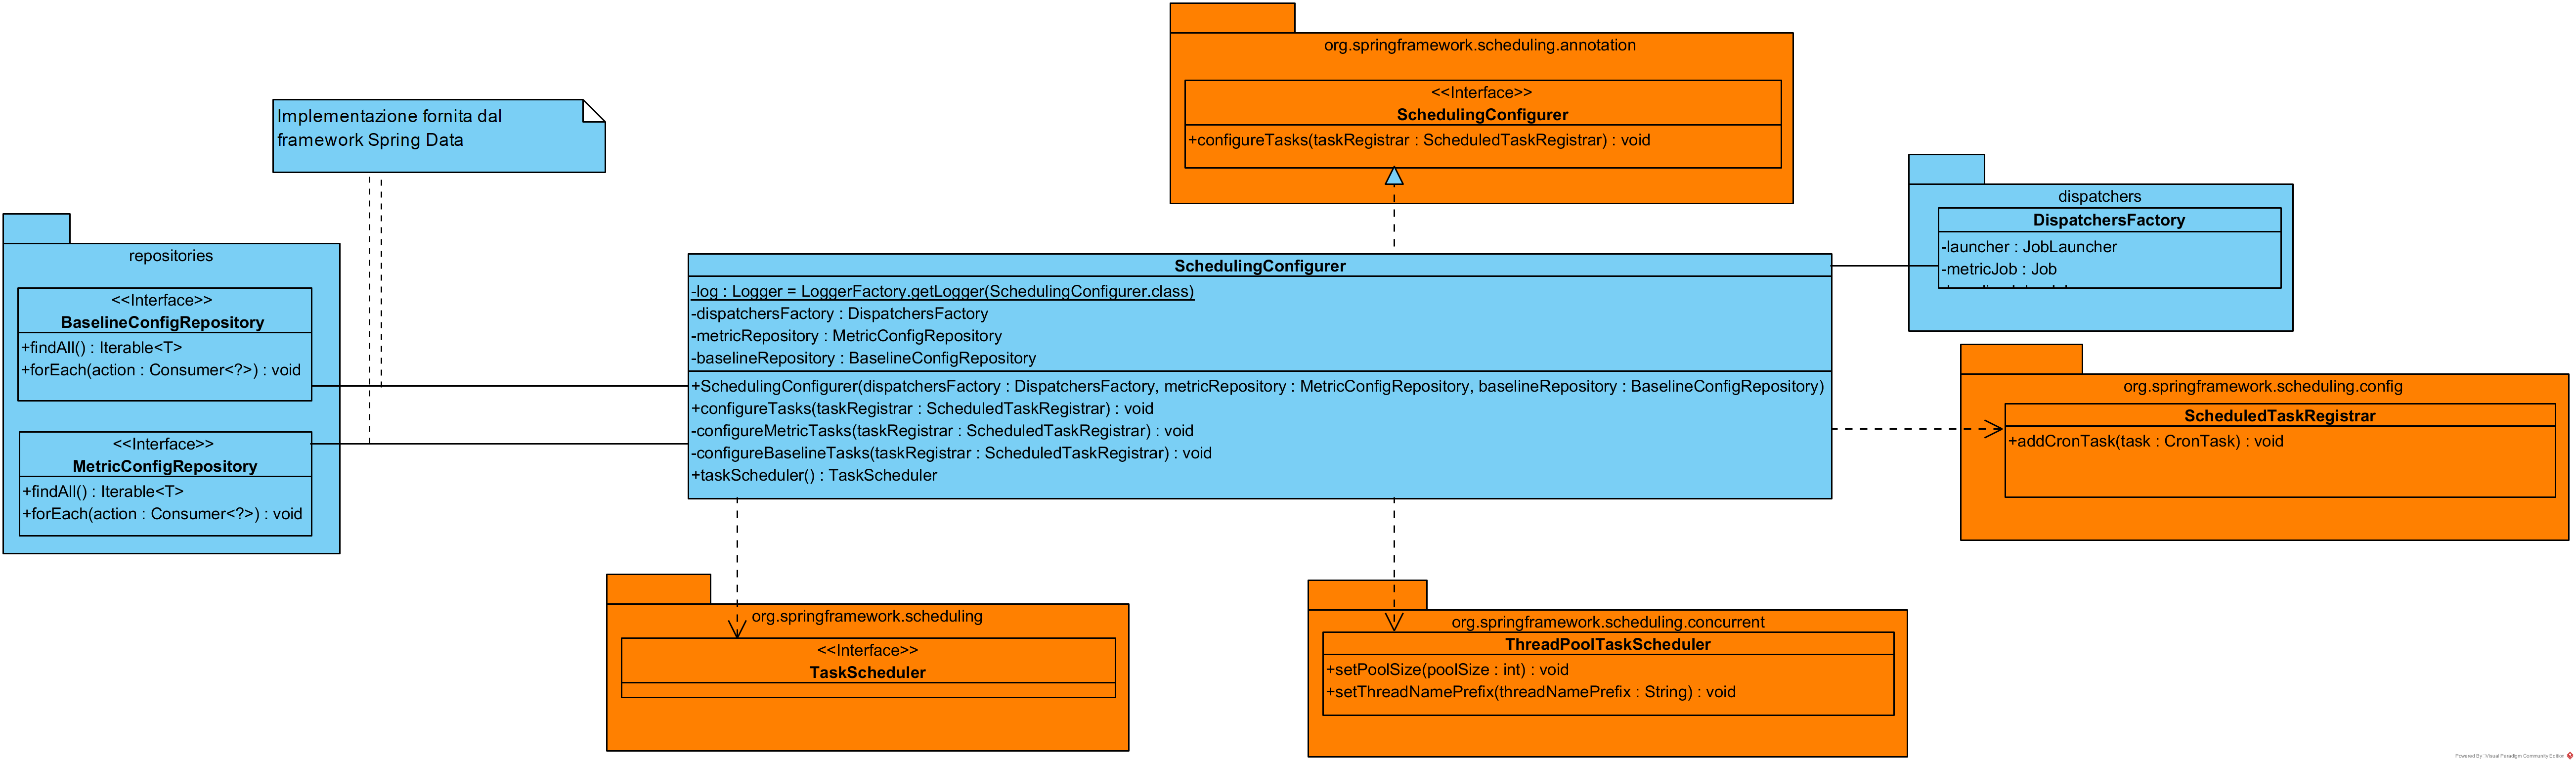
\includegraphics[width=\textwidth]{./img/DiagrammiClasse/SchedulingConfigurer.png}
            \caption[Diagramma della classe SchedulingConfigurer]{Diagramma della classe SchedulingConfigurer}
        \end{figure}
        La classe SchedulingConfigurer:
        \begin{itemize}
        	\item costruisce un oggetto \textit{DispatchersFactory} necessario per la costruzione di dispatchers;
        	\item costruisce un oggetto \textit{MetricConfigRepository} necessario per andare a prelevare da 
        		Elasticsearch la corretta configurazione per le metriche da creare;
        	\item costruisce un oggetto \textit{BaselineConfigRepository} necessario per andare a prelevare da 
        		Elasticsearch la corretta configurazione per le baseline da creare;
        	\item definire un oggetto \textit{TaskScheduler} necessario per la gestione dei \glossaryItem{task} riguardanti
        		le metriche e le baseline all'interno dell'applicazione.
        \end{itemize}
        La classe implementa l'interfaccia \textit{SchedulerConfigurer} del framework Spring. Questo perché permette
        di creare un oggetto \textit{TaskScheduler} capace di aggiungere operazioni alla coda delle operazioni da svolgere.\\
        La classe utilizza le seguenti classi/interfacce:
        \begin{itemize}
        	\item \textbf{DispatchersFactory}: grazie a questa classe è possibile creare dispatchers che gestiscano la coda
        		dei processi;
        	\item \textbf{BaselineConfigRepositories}: permette di prelevare da Elasticsearch la configurazione prevista
        		per la costruzione di una baseline;
        	\item \textbf{MetricConfigRepositories}: permette di prelevare da Elasticsearch la configurazione prevista
        		per la costruzione di una metrica;
        	\item \textbf{TaskScheduler}: questa classe permette la programmazione di oggetti \textit{Runnables} in
        		base a diversi tipi di triggers;
        	\item \textbf{ThreadPoolTaskScheduler}: questa classe è l'implementazione dell'interfaccia \textit{TaskScheduler} 
				utilizzata in \ProjectName{};
        	\item \textbf{SchedulerTaskRegistrar}: è utilizzata come classe di supporto nella registrazione di 
        		operazioni nel \textit{TaskScheduler}.
        \end{itemize}

\newpage

   \subsection{Package dispatchers}

        \begin{figure}[htbp]
            \centering
            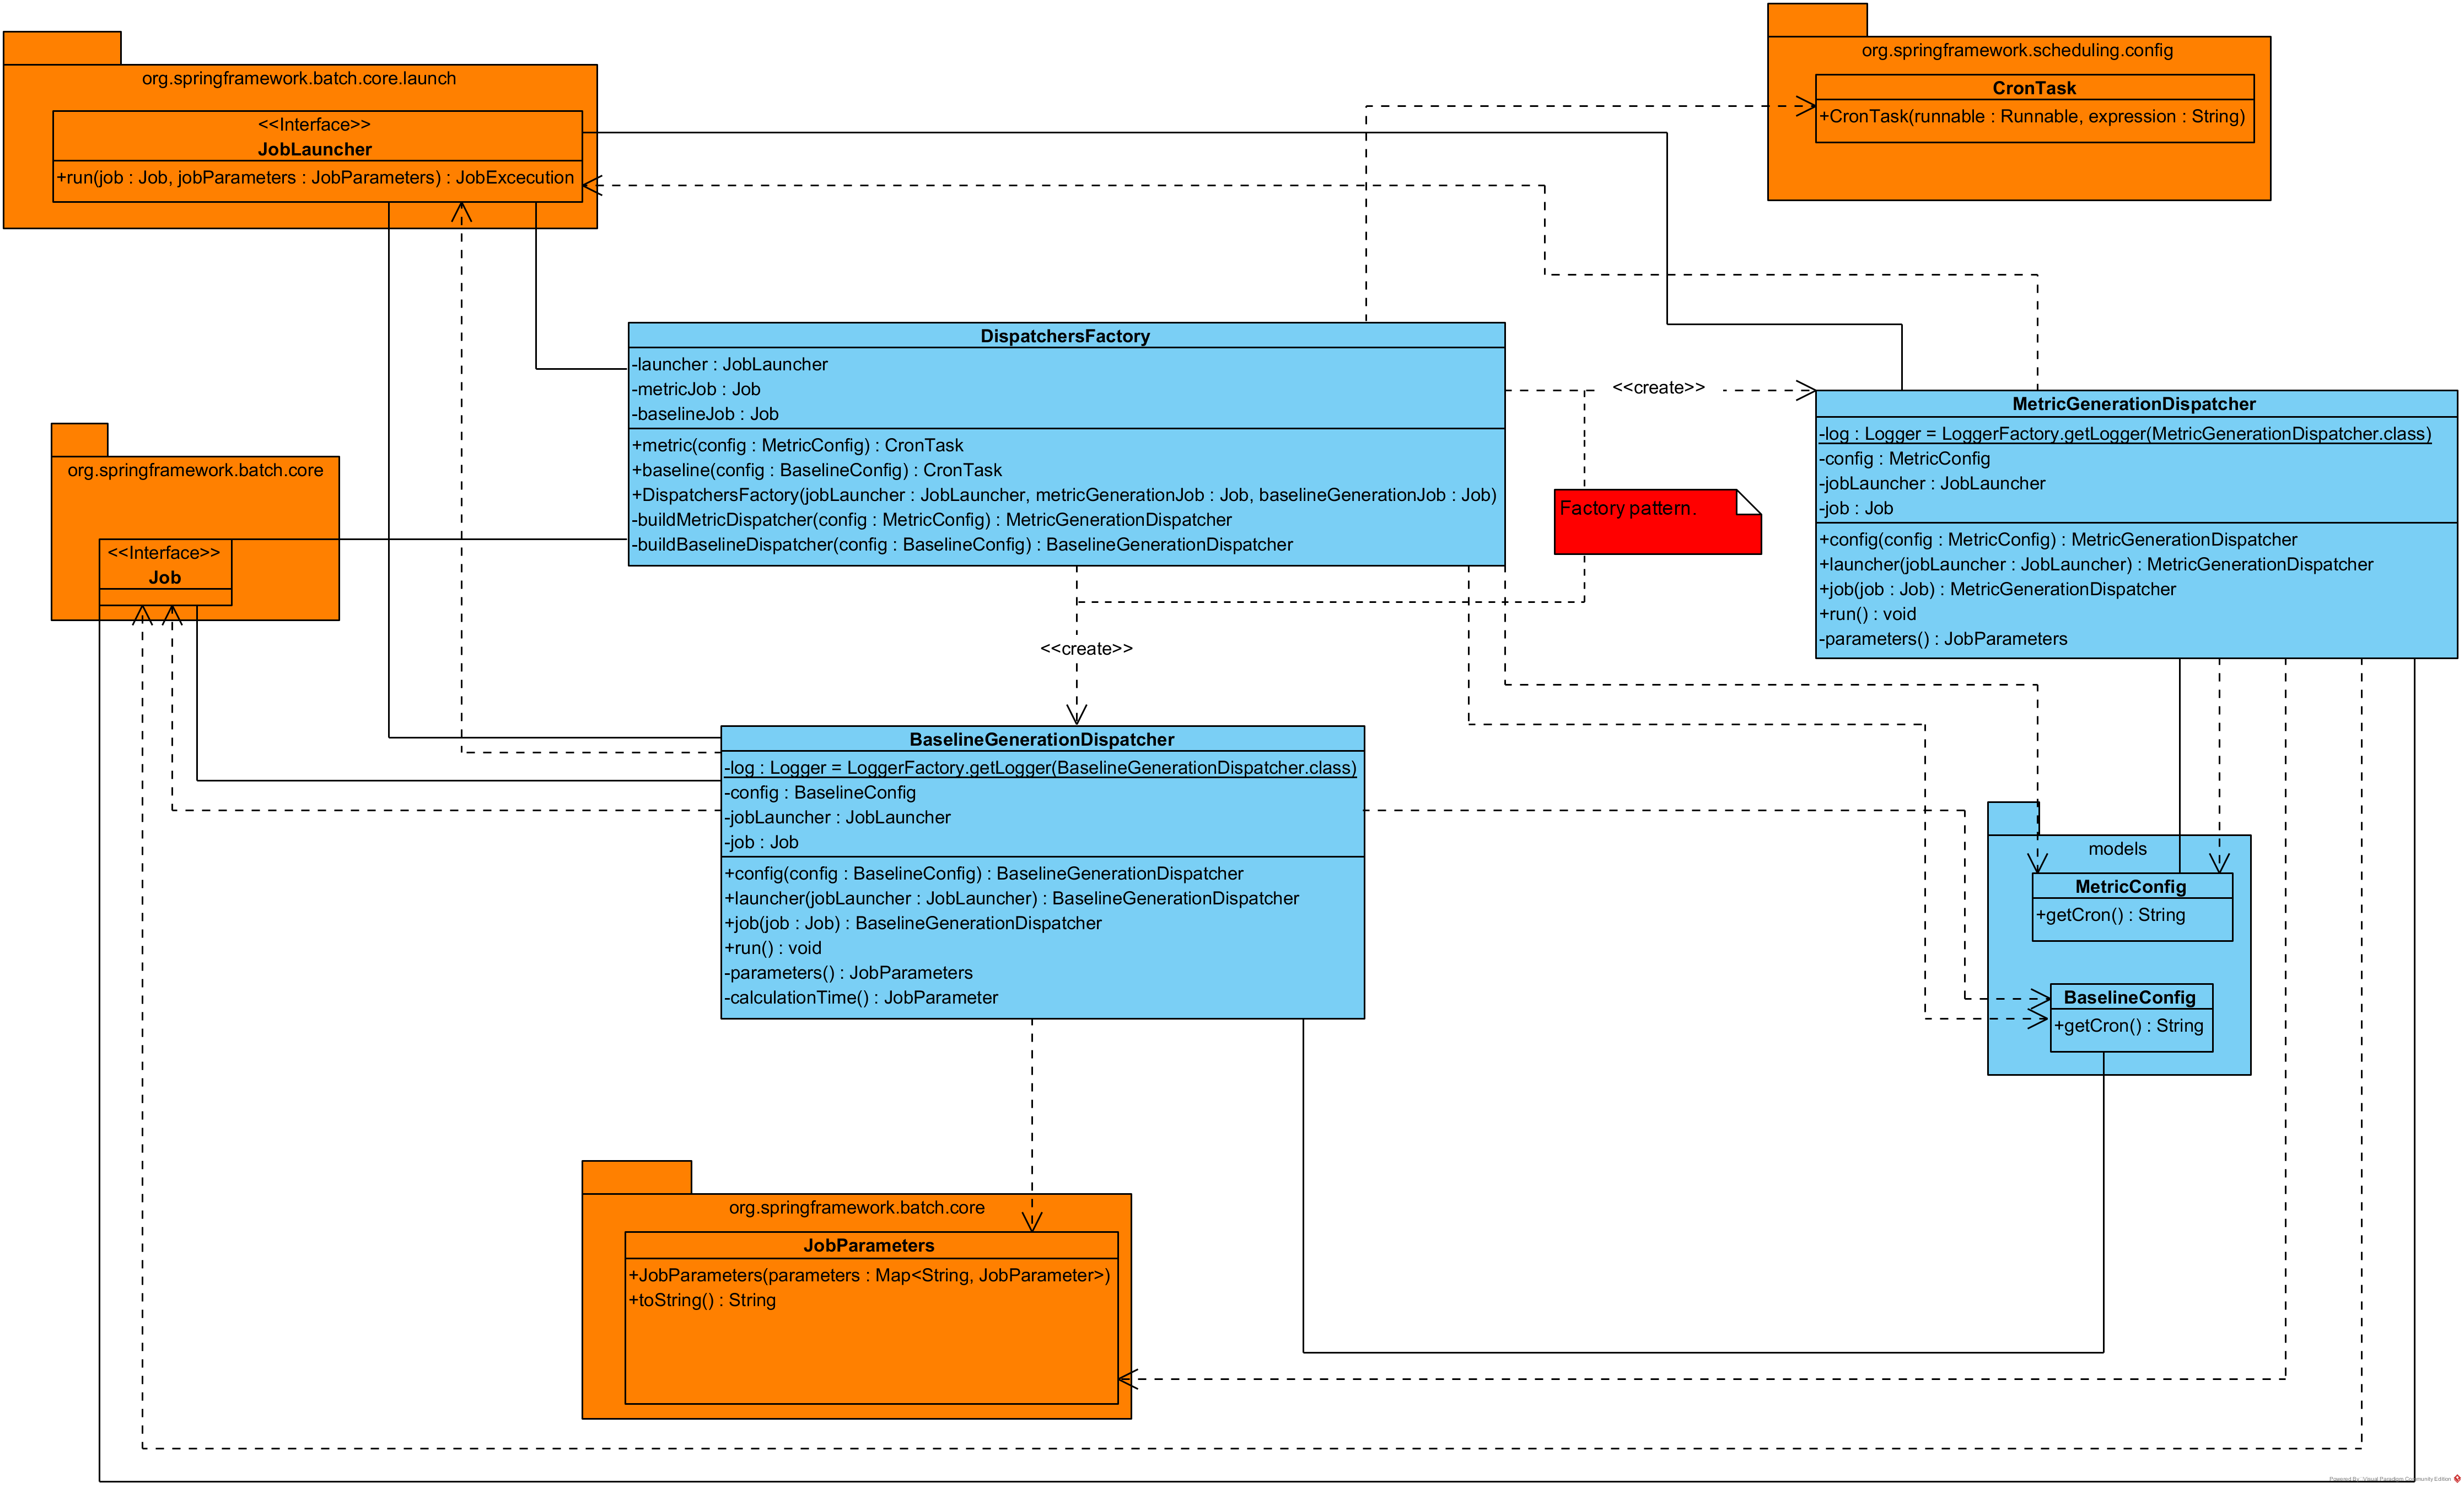
\includegraphics[width=\textwidth]{./img/DiagrammiClasse/dispatchers.png}
            \caption[Diagramma del package dispatchers]{Diagramma del package dispatchers}
        \end{figure}
        Il diagramma rappresenta il package dispatchers, composto dalle seguenti classi:
        \begin{itemize}
        	\item \textbf{DispatchersFactory}: questa classe permette la creazione di dispatchers in base ad una
        		configurazione data in input lasciando alle sotto-classi l'implementazione effettiva, si basa infatti
        		sul factory pattern;
        	\item \textbf{BaselineGenerationDispatcher}: questa classe rappresenta un disparcher per la generazione
        		di baseline basate sulle metriche prodotte nell'ultima ora;
        	\item \textbf{MetricGenerationDispatchers}: questa classe rappresenta un disparcher per la generazione
        		di metriche basante sulle traces raccolte dall'ora attuale fino ad un tempo indicato dalla strategia
        		scelta.
        \end{itemize}
\newpage

    \subsection{Package jobs}

        \begin{figure}[htbp]
            \centering
            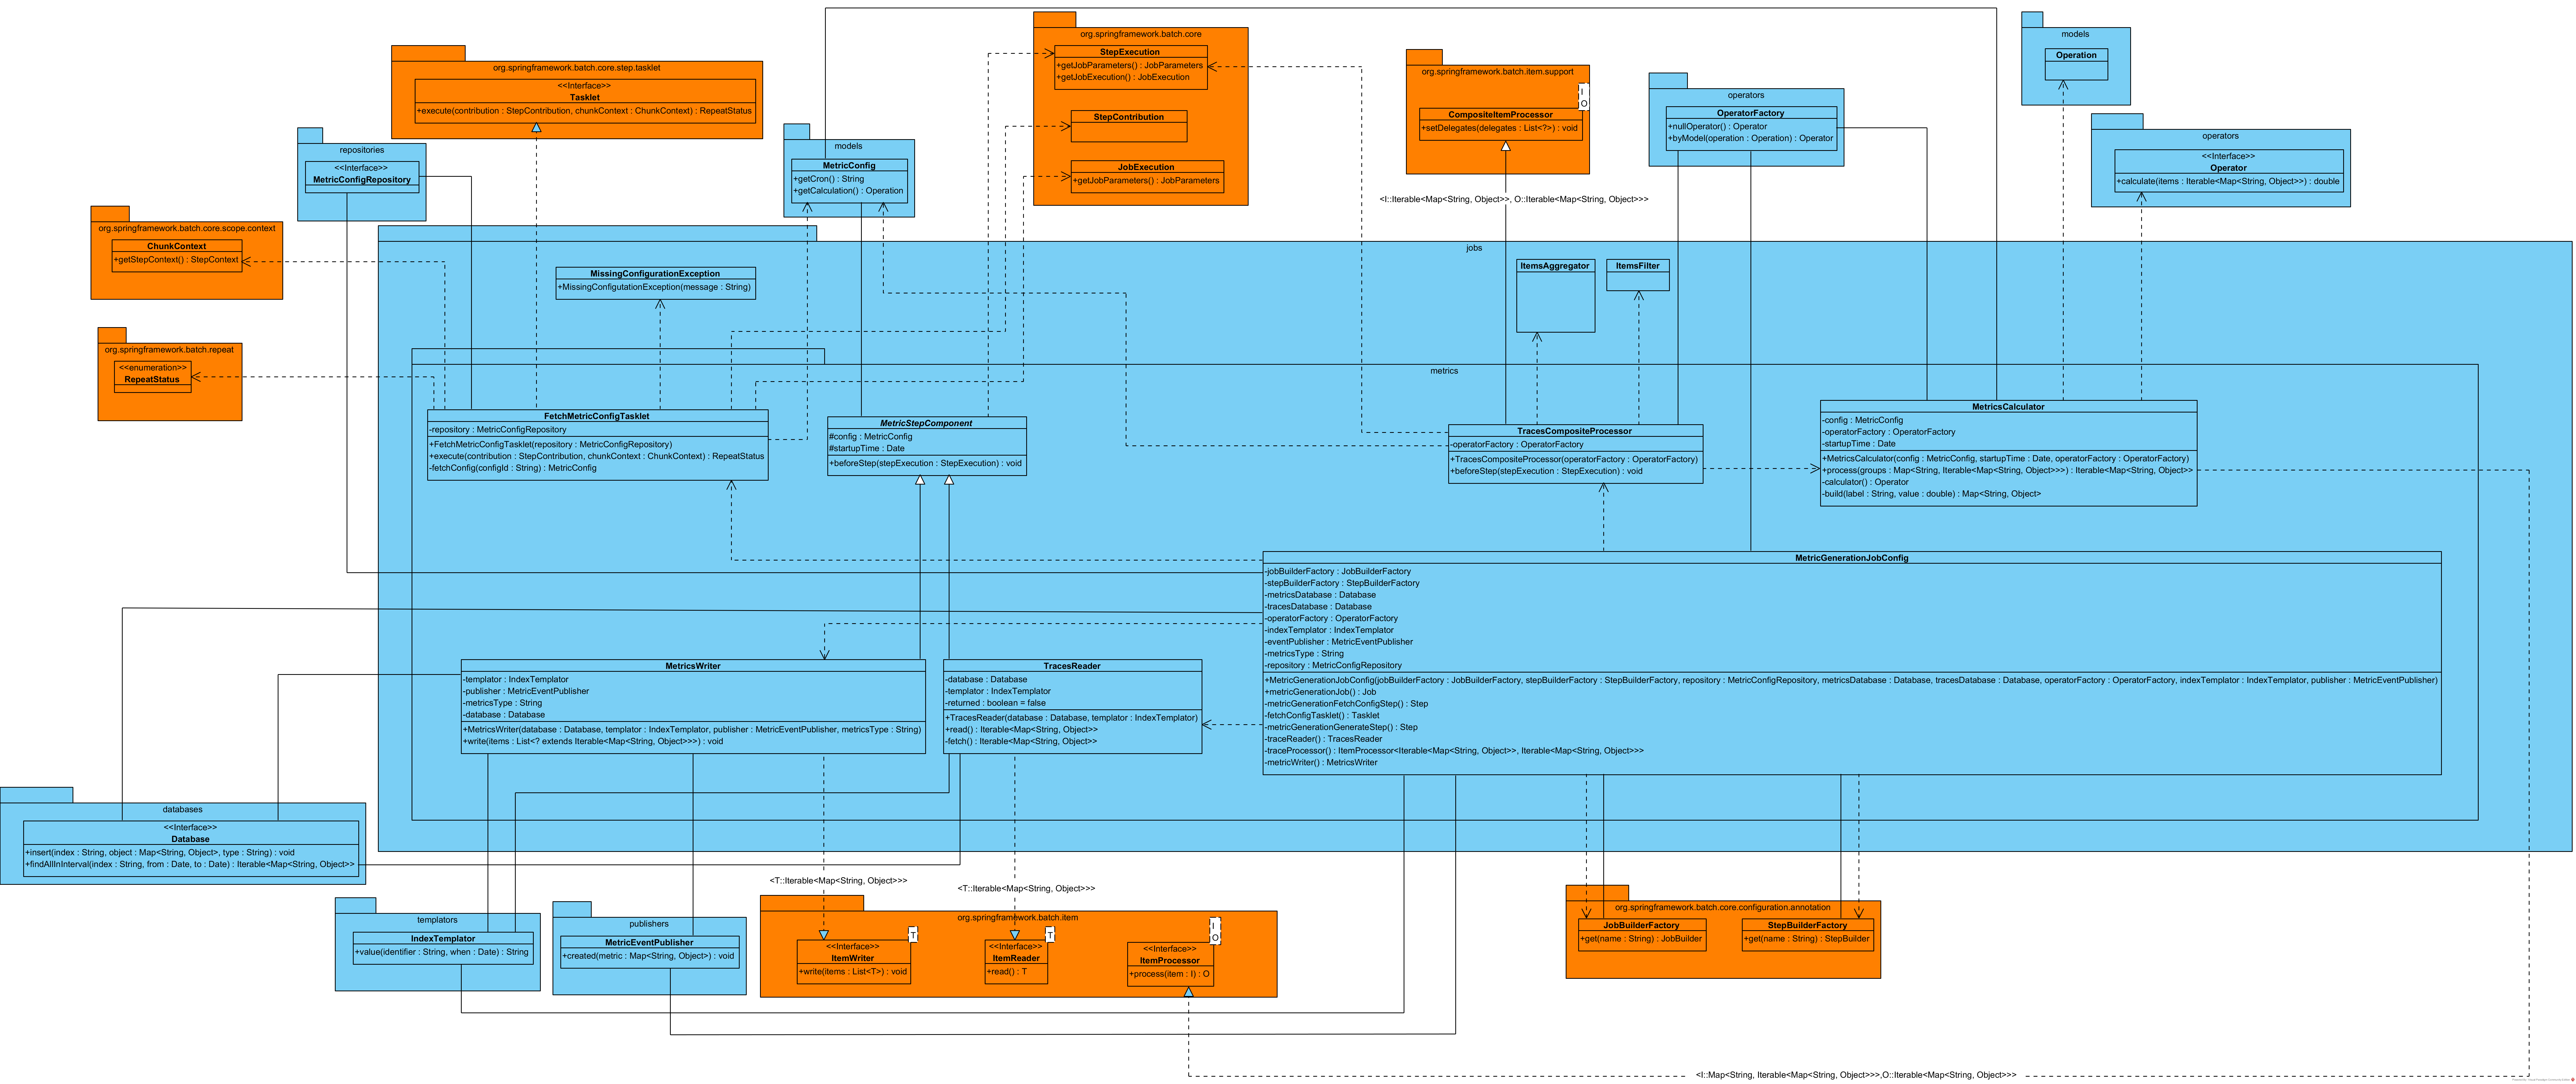
\includegraphics[width=\textwidth]{./img/DiagrammiClasse/metricJob.png}
            \caption[Diagramma di jobs - metric]{Diagramma della parte sulle metriche del package jobs}
        \end{figure}
        Il diagramma rappresenta il compito di generare una metrica. Vi è un diagramma equivalente per le baseline, non presentato
        perché simile. Il package jobs, per la parte dedicata alle metriche, è composto dalle seguenti classi:
        \begin{itemize}
        	\item \textbf{FetchMetricConfigTasklet}: classe che preleva dal database la configurazione per la 
        		creazione delle metriche basandosi su un identificatore; essa può lanciare una 
        		\textit{MissingConfigurationException} in caso la configurazione sia presente nel database;
        	\item \textbf{MetricStepComponent}: classe astratta che permette di prelevare dei parametri dal contesto 
        		di un lavoro prima dell'esecuzione dello stesso;
        	\item \textbf{MetricsWriter}: implementazione di \textit{MetricStepComponent} che permette di salvare
        		la metriche prodotte nel database;
        	\item \textbf{TracesReader}: implementazione di \textit{MetricStepComponent} che permette di leggere
        		le traces presenti nel database;
        	\item \textbf{TracesCompositeProcessor}: questa classe definisce una serie di processori coinvolti
        		nella generazione di metriche a partire da traces, questa classe è necessaria per sapere 
        		se è presente un evento di tipo \textit{BeforeStep};
        	\item \textbf{MetricGenerationJobConfig}: questa classe rappresenta la configurazione per l'operazione
        		di creazione di metriche a partire da traces;
        	\item \textbf{MetricsCalculator}: questa classe permette il calcolo di una metrica a partire da un 
        		insieme di traces in input;
        	\item \textbf{ItemsAggregator}: classe che aggrega tutti gli input suddivisi in gruppi in base 
        		ad una configurazione data;
        	\item \textbf{ItemsFilter}: classe che filtra tutti gli input in base ad una configurazione data;
        	\item \textbf{MissingConfigurationException}: eccezione che indica che il compito indicato in 
        		input non è presente nel database.
        \end{itemize}

\newpage

    \subsection{Diagramma Metric - Alert}

        \begin{figure}[htbp]
            \centering
            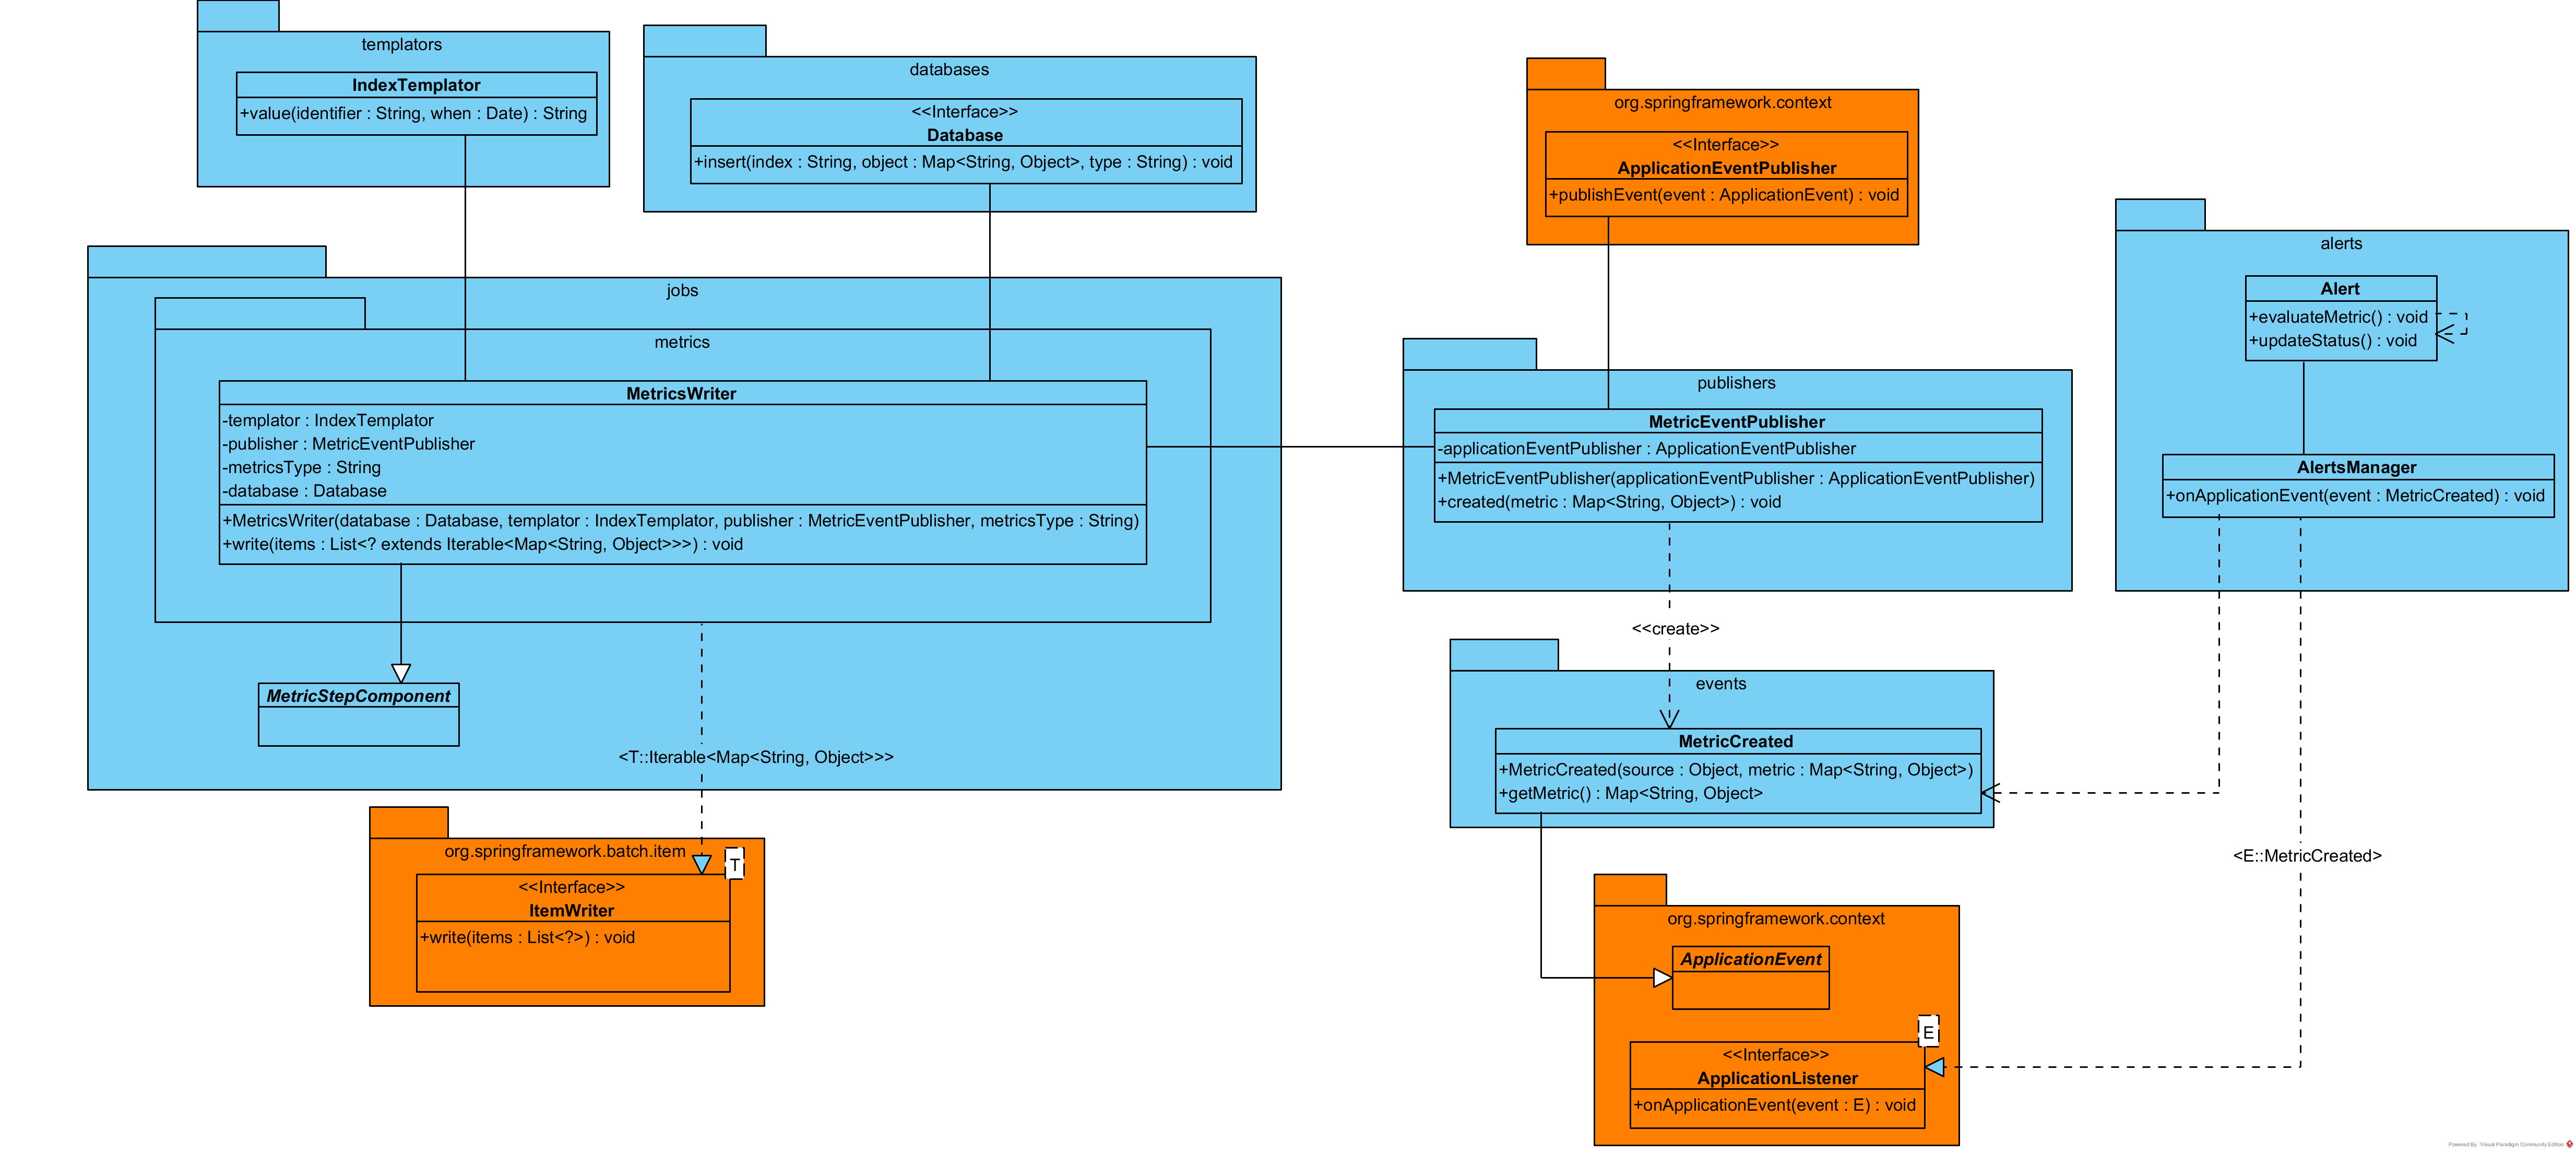
\includegraphics[width=\textwidth]{./img/DiagrammiClasse/metricToAlert.png}
            \caption[Diagramma Metric - Alert]{Diagramma che mostra l'interazione tra il package metric e il package alert}
        \end{figure}
        Il diagramma rappresenta l'interazione tra il package metric e il package alert. \\
	Al momento della creazione di una metrica viene lanciato un evento MetricCreated e vengono controllate le condizioni degli alert per tale metrica. \\
        Le classi più importanti sono:
        \begin{itemize}
        	\item \textbf{MetricsWriter}: essa scrive nel database una nuova metrica con il metodo \\
        		\verb=void write(List<? extends Iterable<Map<String, Object>>>)= utilizzando un \textit{IndexTemplator} 
        		per il nuovo indice;
        	\item \textbf{MetricEventPublisher}: una volta creata una nuova metrica, essa notifica questo evento
        	\item \textbf{MetricCreated}: rappresenta l'evento di creazione di una metrica ed è un'estensione
        		di un \textit{ApplicatioEvent}, questo per far si che un \textit{ApplicationListener}, nel prodotto esteso
        		dalla classe \textit{AlertsManager}, possa rimanere in ascolto di tutti gli eventi accaduti;
        	\item \textbf{AlertsManager}: gestisce gli alert dei prodotti in base agli eventi accaduti, rimanendo in ascolto di oggetti \textit{MetricCreated}, controllandole successivamente gli alerts necessari.
        \end{itemize}

\newpage


        \subsection{Sotto-package evaluators}

            \begin{figure}[htbp]
                \centering
                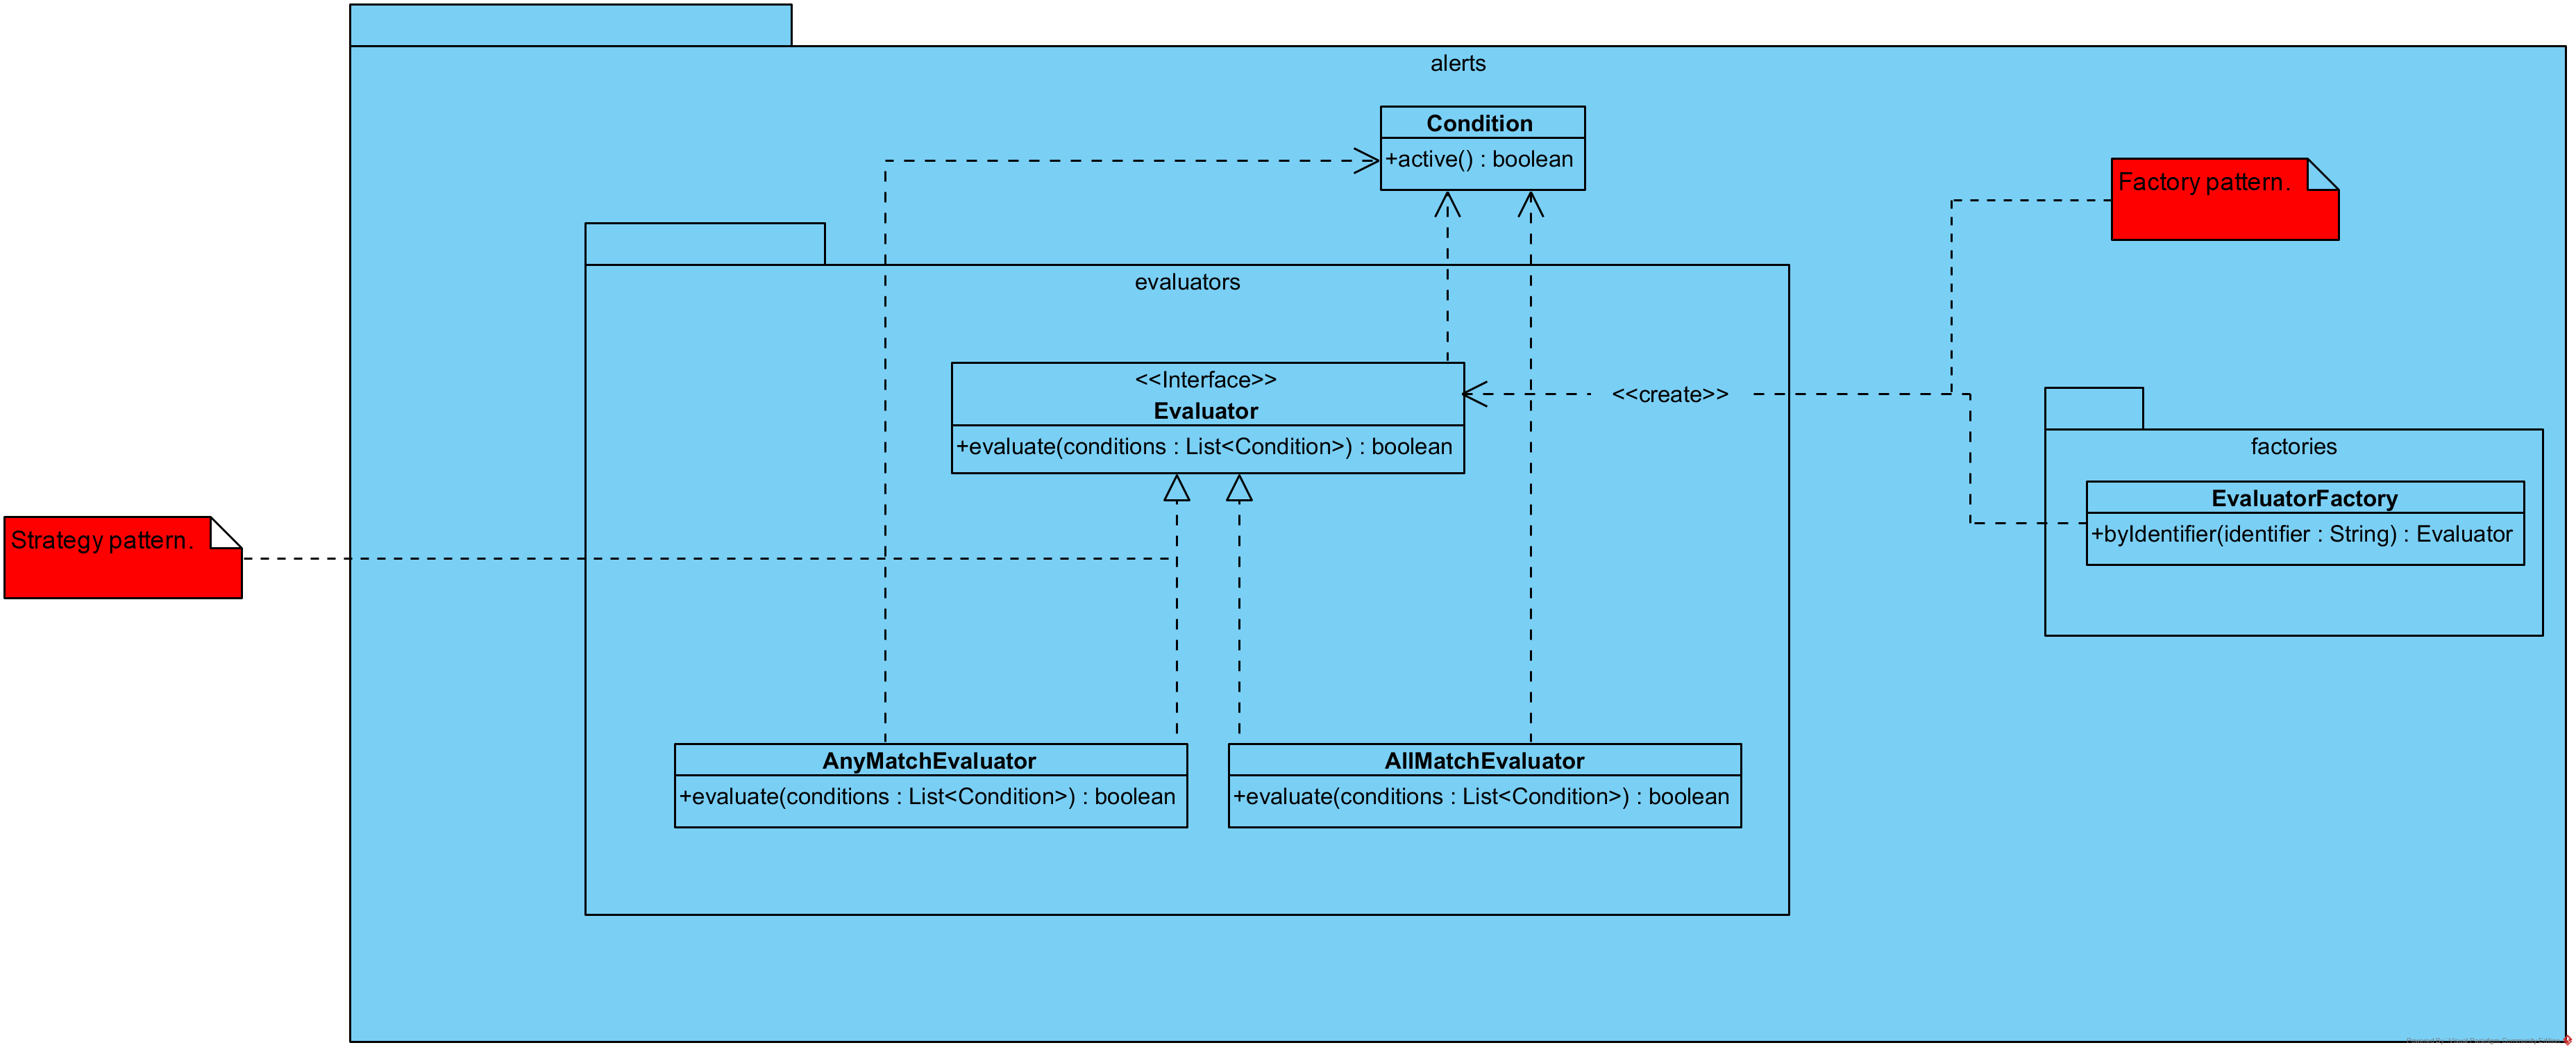
\includegraphics[width=\textwidth]{./img/DiagrammiClasse/evaluators.png}
                \caption[Diagramma del package alerts.evaluators]{Diagramma del package alerts.evaluators}
            \end{figure}
            Il diagramma rappresenta il sotto-package evaluators del package alerts. Un evaluator controlla se 
            le conditions per l'alert sono soddisfatte, generando in caso un critical event.\\
            Vengono di seguito spiegate alcune classi ed interfacce:
            \begin{itemize}
            	\item \textbf{Evaluator}: interfaccia che rappresenta un oggetto il quale riceve una serie 
            		di condizioni in input e, a seconda della politica adottata, decide se è 
            		necessario lanciare un'azione di rimedio. Anche in queste classi, come in \textit{Action}, 
            		è stato scelto di utilizzare lo strategy pattern per separare l'implementazione della politica
            		di valutazione con il client che lo utilizza;
            	\item \textbf{Condition}: questa classe rappresenta una condizione che, se vera,
            		indica la necessità del lancio di un'azione di rimedio. Una lista di queste condizioni viene analizzata da un \textit{Evaluator};
            	\item \textbf{EvaluatorFactory}: questa classe permette di costruire un valutatore basandosi 
            		su una configurazione data; per far ciò si è scelto di utilizzare il factory pattern, come 
            		in \textit{ActionFactory}, per dare la responsabilità dell'implementazione del valutatore 
            		corretto alle sue sotto-classi.
            \end{itemize}

\newpage

    \subsection{Sottopackage verifiers}

        \begin{figure}[htbp]
            \centering
            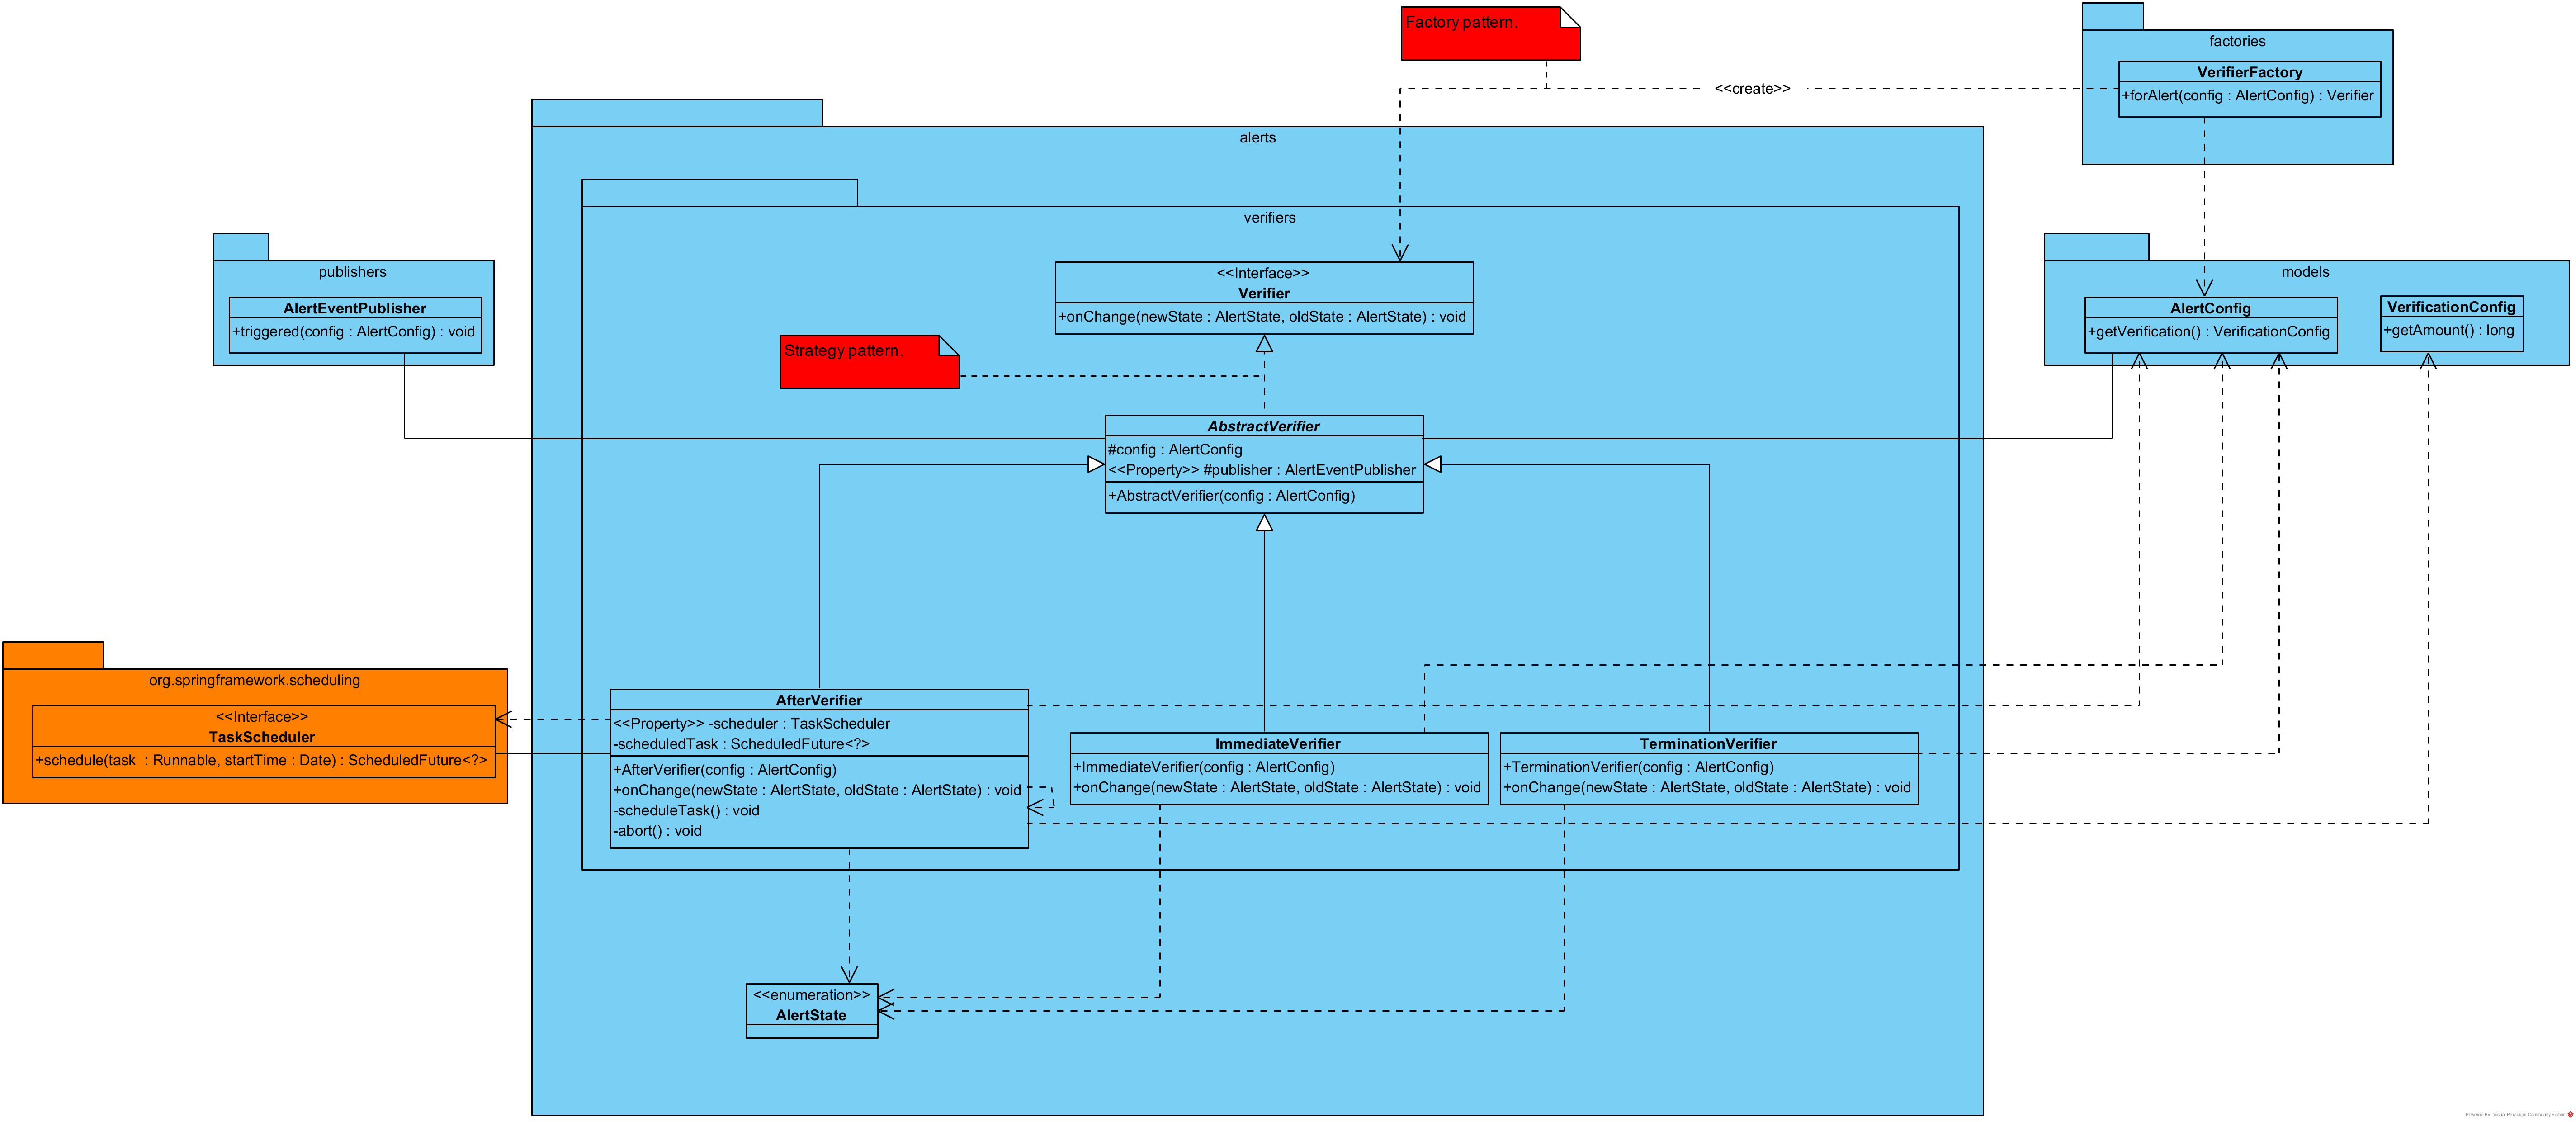
\includegraphics[width=\textwidth]{./img/DiagrammiClasse/verifiers.png}
            \caption[Diagramma del sottopackage verifiers]{Diagramma del sottopackage verifiers}
        \end{figure}
        Il diagramma rappresenta il package verifiers, sottopackage di alerts. I verificatori servono a
        porre una condizione sul lancio di un'azione di rimedio, infatti questa classe riceve in input uno 
        stato per un alert e decide se o quando lanciare un'azione di rimedio.\\
        Il package è composto dalle seguenti classi/interfacce:
        \begin{itemize}
        \item \textbf{Verifier}: interfaccia per un verificatore, questa astrazione permette di separare
        	il client che utilizza l'oggetto dall'implementazione effettiva di questo, seguendo l'organizzazione
        	delle classi del pattern strategy;
        \item \textbf{AbstractVerifier}: classe astratta per un verificatore;
        \item \textbf{AfterVerifier}: verificatore che lancia un'azione di rimedio dopo alcuni secondi il 
        	verificarsi del cambio di stato dell'alert;
        \item \textbf{ImmediateVerifier}: verificatore che lancia un'azione di rimedio non appena si verifica 
        	un cambio di stato dell'alert;
        \item \textbf{TerminationVerifier}: verificatore che lancia un'azione di rimedio dopo che l'evento 
        	scatenante l'alert sia terminato;
        \item \textbf{AlertState}: classe che descrive tutti i possibili stati di un alert;
        \item \textbf{VerifierFactory}: classe che permette di costruire un verificatore in base ad una 
        		configurazione scelta, è stato scelto di organizzare l'architettura di questa classe
        		seguendo il factory pattern, già descritto precedentemente;
        \end{itemize}

\newpage

   \subsection{Diagramma Alerts - Actions}

        \begin{figure}[htbp]
            \centering
            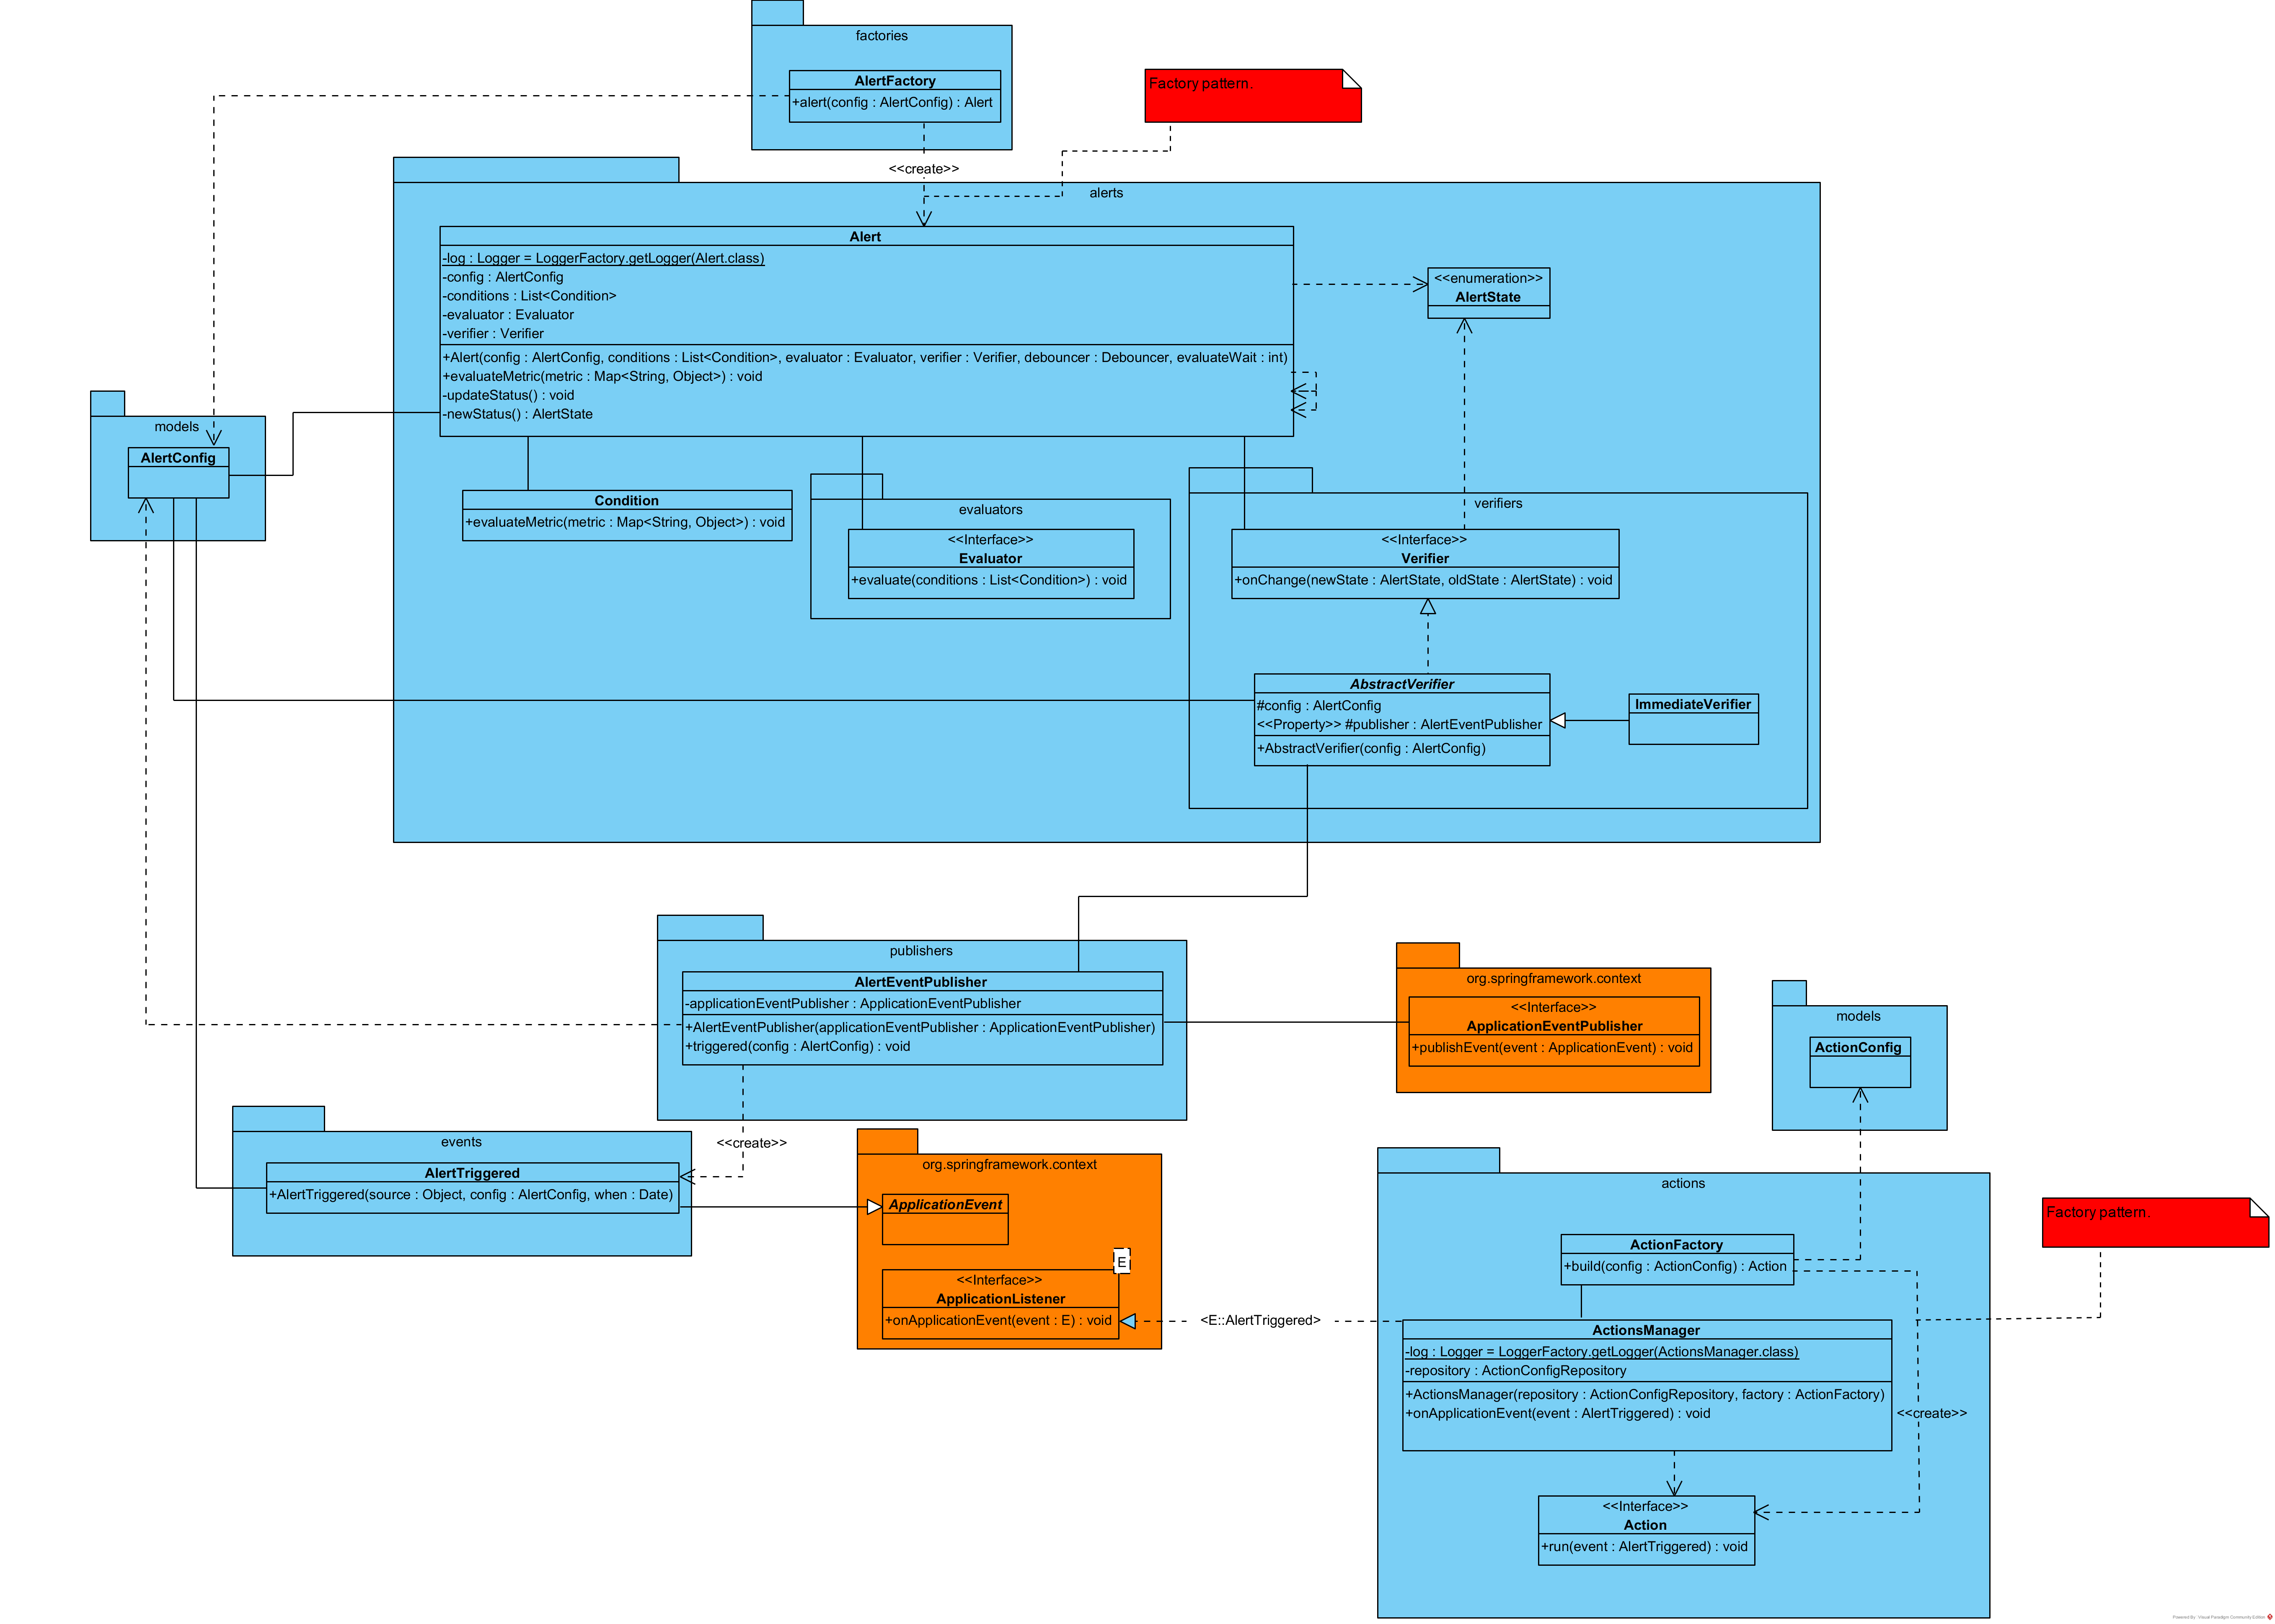
\includegraphics[width=\textwidth]{./img/DiagrammiClasse/alertToAction.png}
            \caption[Diagramma alert - actions]{Diagramma che mostra l'interazione tra alerts e actions}
        \end{figure}
        Il diagramma di classe mostra le dipendenze tra il package alerts e il package actions. Si è deciso di creare tale diagramma per
        comprendere quali classi agiscono nell'interazione tra i due packages. \\
        Interazioni:
        \begin{itemize}
        	\item \textbf{Alert - Verifier}: l'oggetto \textit{Verifier}, alla notifica di un evento, andrà a modificare 
        		\textit{AlertStatus} secondo la sua politica attraverso il metodo \verb=void onChange(AlertState, AlertState)=, 
        		causando così lo scattare di un \textit{Alert};  
        	\item \textbf{AbstractVerifier - AlertEventPublisher}: l'oggetto \textit{AlertEventPublisher} è responsabile
        		della notifica ad un \textit{AbstractVerifier} del verificarsi di un evento, quest'ultimo, o meglio
        		l'implementazione scelta di quest'ultimo, va a decide se e quando lanciare un'azione di rimedio;
        	\item \textbf{AlertEventPublisher - AlertTriggered}: allo scattare di un alert, \textit{AlertEventPublisher}
        		crea un oggetto \textit{AlertTriggered} che rappresenta l'evento di un alert scattato;
        	\item \textbf{ActionsManager - AlertTriggered}: allo scattare di un alert, quindi alla creazione di un
        		\textit{AlertTriggered}, l'oggetto di tipo \textit{ActionsManager}, che rimane in ascolto di eventi
        		di tipo \textit{AlertTriggered} tramite \textit{ApplicationListener}, gestisce le azioni di rimedio
        		da utilizzare.
        \end{itemize}

\newpage

    \subsection{Package actions}

        \begin{figure}[htbp]
            \centering
            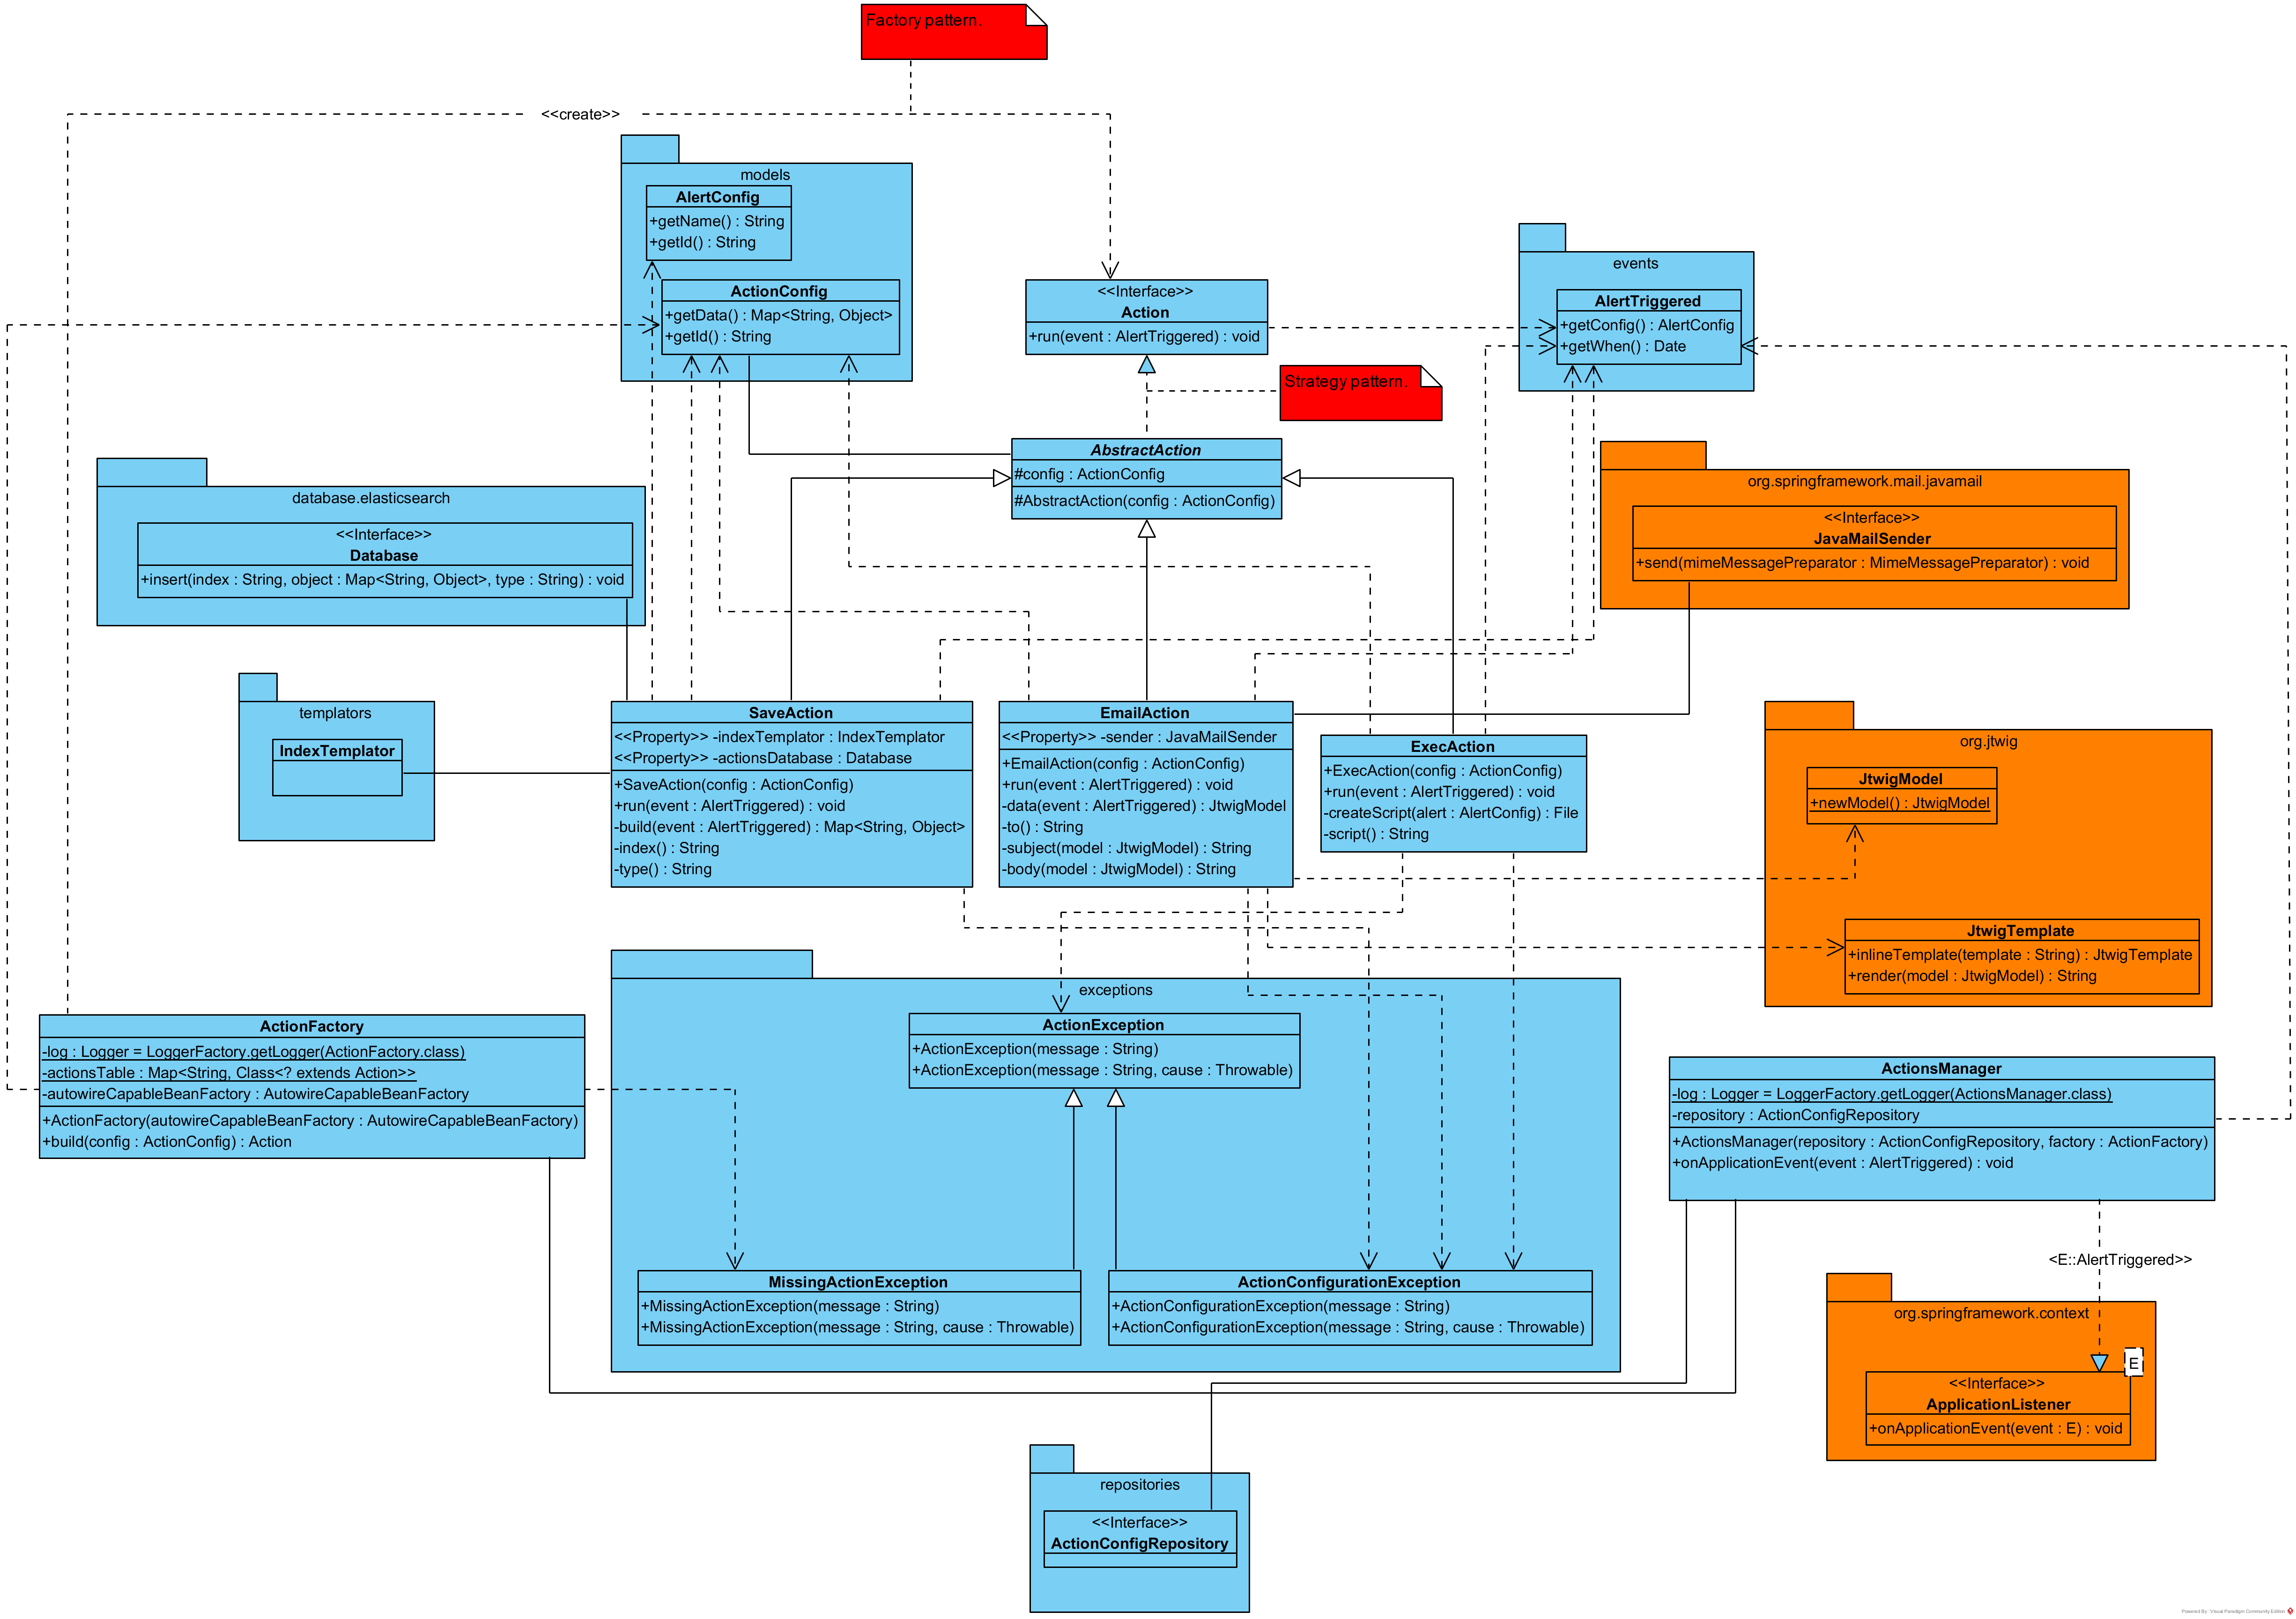
\includegraphics[width=\textwidth]{./img/DiagrammiClasse/actions.png}
            \caption[Diagramma del package actions]{Diagramma del package actions}
        \end{figure}
        Il diagramma di classe rappresenta il package actions, diviso nelle seguenti parti:
        \begin{itemize}
        	\item \textbf{Action}: interfaccia rappresentante un'azione di rimedio, nella costruzione di 
        		queste classi si è deciso di utilizzare il pattern strategy, cioè creando un'interfaccia 
        		che non implementi le azioni da svolgere e lasciando questo compito alle sotto-classi. 
        		Questo permette rendere indipendente l'algoritmo utilizzato nell'azione di rimedio dal
        		client che la utilizza;
        	\item \textbf{ActionException}: questa classe permette di gestire anomalie nell'esecuzione e di
        		lanciare un eccezione nel caso un'azione di rimedio non possa essere eseguita, ad esempio
        		se la configurazione desiderata per l'azione non è corretta o se l'azione richiesta non 
        		esiste;
        	\item \textbf{ActionFactory}: questa classe è responsabile della creazione ed utilizza il
        		factory pattern, cioè permette di creare un astrazione nella creazione delle classi 
        		definendo un oggetto astratto e lasciando alle sotto-classi la definizione dell'oggetto;
        	\item \textbf{ActionsManager}: questa classe gestisce la azioni di rimedio nel caso scatti un
        		alert.
        \end{itemize}

\newpage

 
    \subsection{Package databases}

        \begin{figure}[htbp]
            \centering
            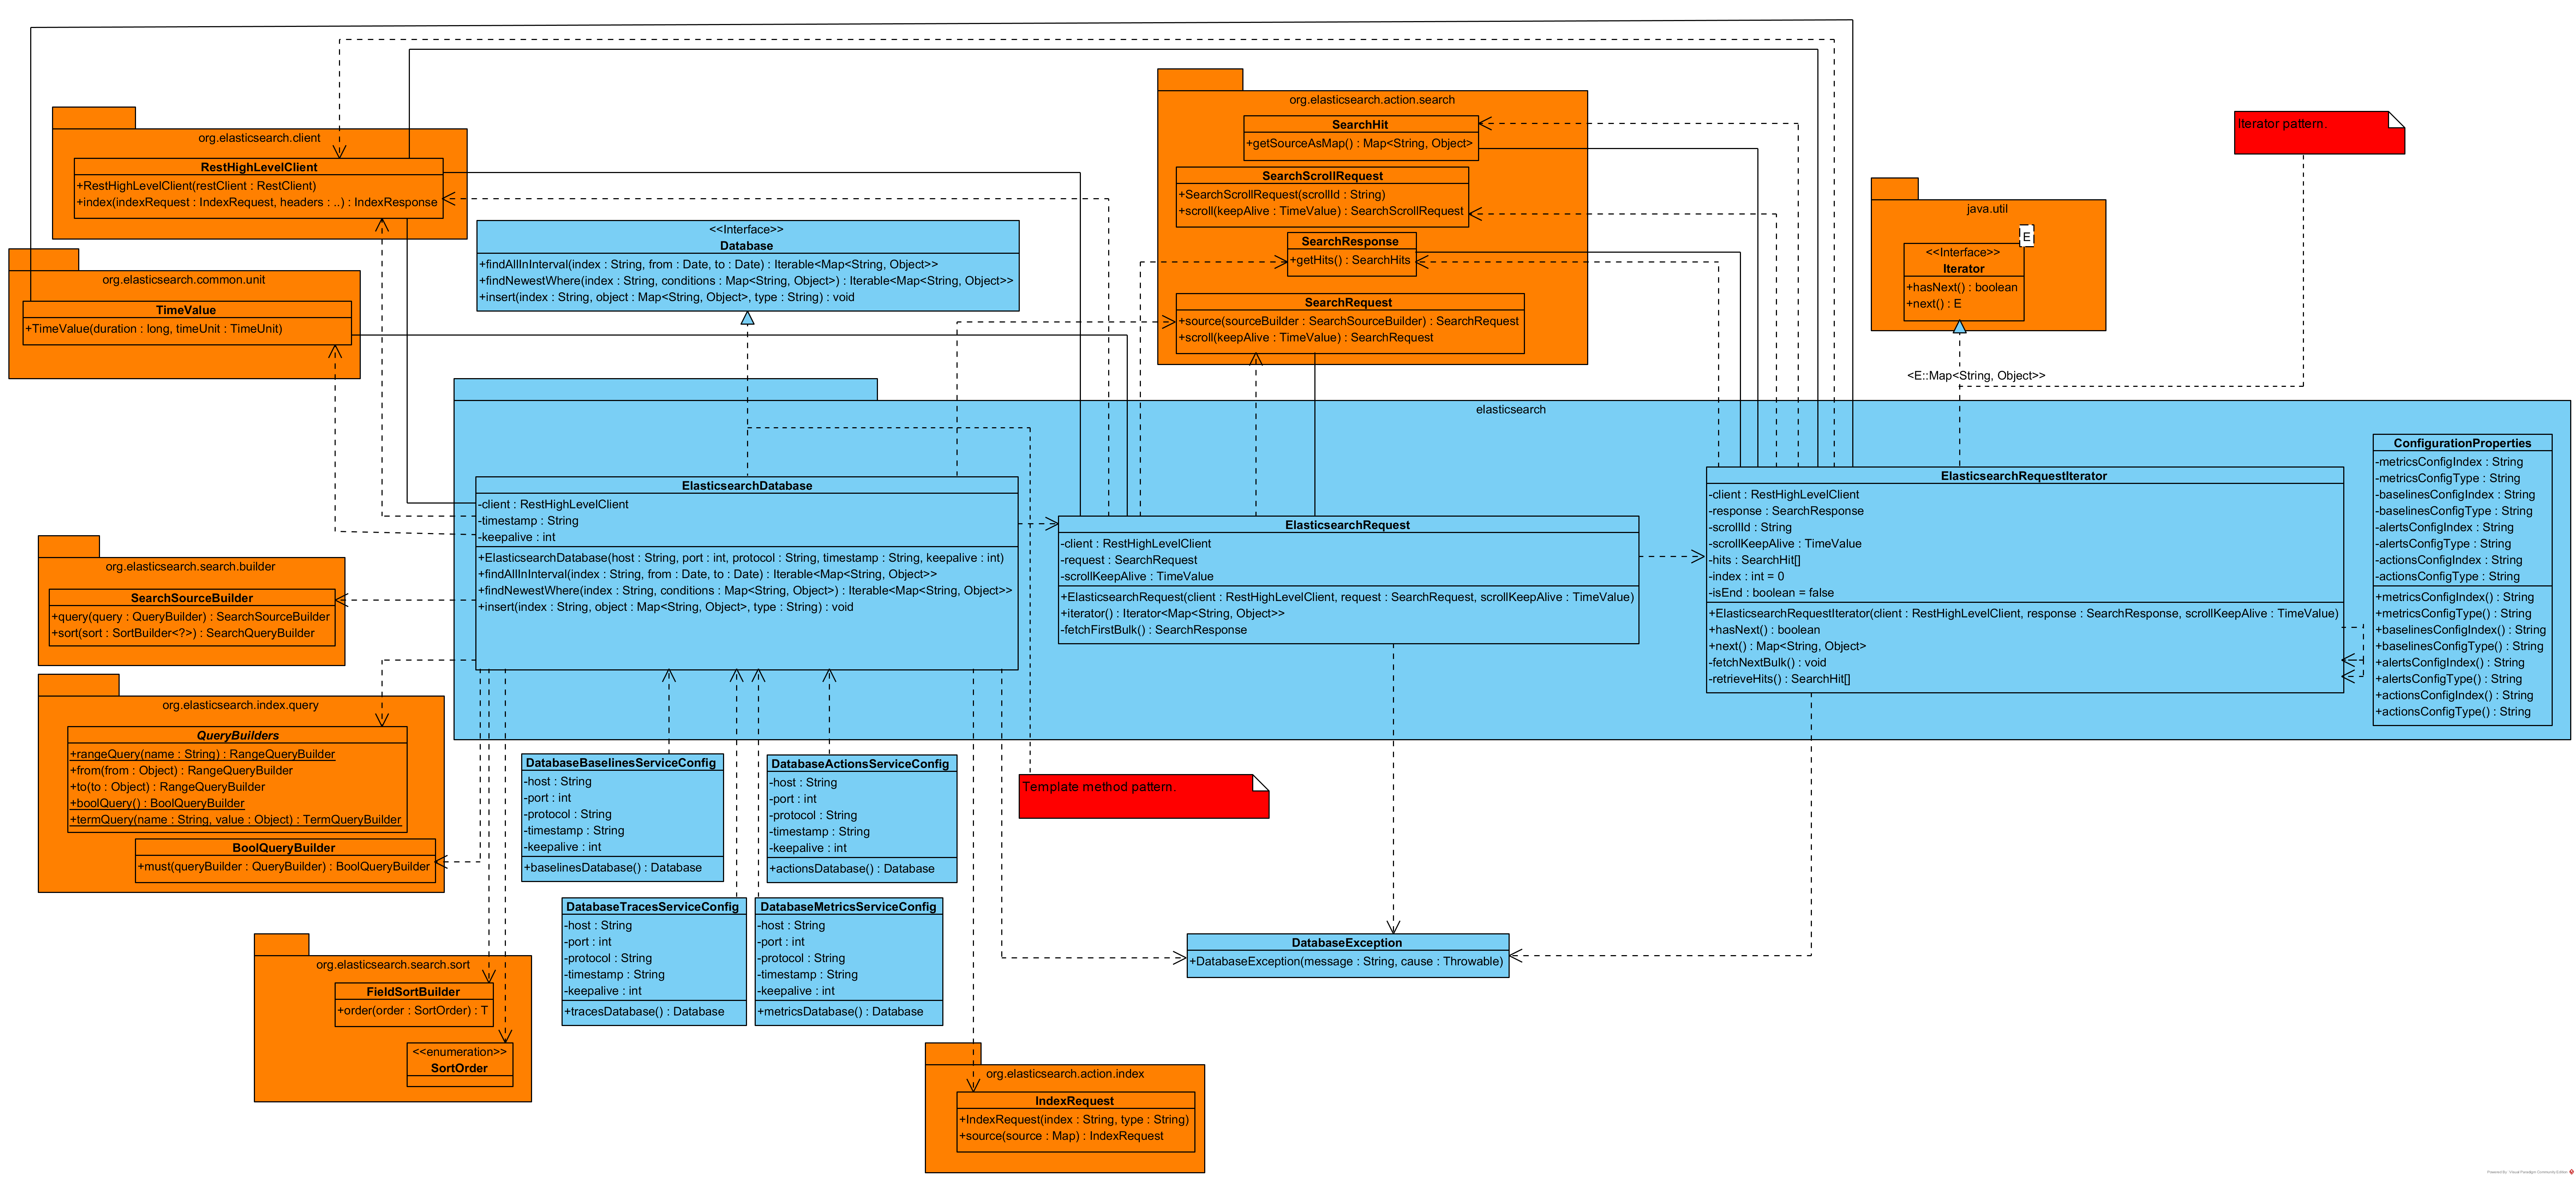
\includegraphics[width=\textwidth]{./img/DiagrammiClasse/databases.png}}
            \caption[Diagramma del package databases]{Diagramma del package databases}
        \end{figure}
        Il diagramma rappresenta il package databases contenente le classi per gestire dati da 
        memorizzare durante l'esecuzione di \ProjectName{}.\\
        Vengono spiegate le seguenti classi/interfacce:
        \begin{itemize}
        	\item \textbf{Databases}: questa interfaccia rappresenta in modo astratto in database necessario
        		alla raccolta di dati utili nell'esecuzione. \GroupName{} ha voluto sviluppare questa classe 
        		utilizzando il template method pattern, cioè creare una classe astratta e lasciare
        		l'implementazione dei metodi alle varie sotto-classi, questo ha reso estendibile il prodotto 
        		ad ulteriori tipi di database, infatti in \ProjectName{} è presente l'implementazione di 
        		questa classe per usare un database con Elasticsearch con la classe \textit{ElasticsearchDatabase};
        	\item \textbf{ElasticSearchIterator}: questa classe permette lo scorrimento dei risultati ottenuti 
        		da una richiesta ad un \textit{ElasticsearchDatabase}, per implementarlo \GroupName{} ha secuito
        		l'iterator pattern, creando così un iteratore che tenga traccia della posizione corrente e calcoli 
        		il prossimo elemento così da poter attraversare tutti gli elementi ottenuti dal database;
        	\item \textbf{ConfigurationProperties:} viene utilizzata questa classe per configurare i metadati del 
        		container IoC di Spring anziché farlo tramite XML, in particolare le proprietà descritte nel file
        		 ``application.properties'' vengono legate ad un corrispettivo Bean affinché le si possano risolvere 
        		 nelle annotazioni quando si voglia far uso di Dependency Injection.
        \end{itemize}

\newpage

 

    \subsection{Package operators}

        \begin{figure}[htbp]
            \centering
            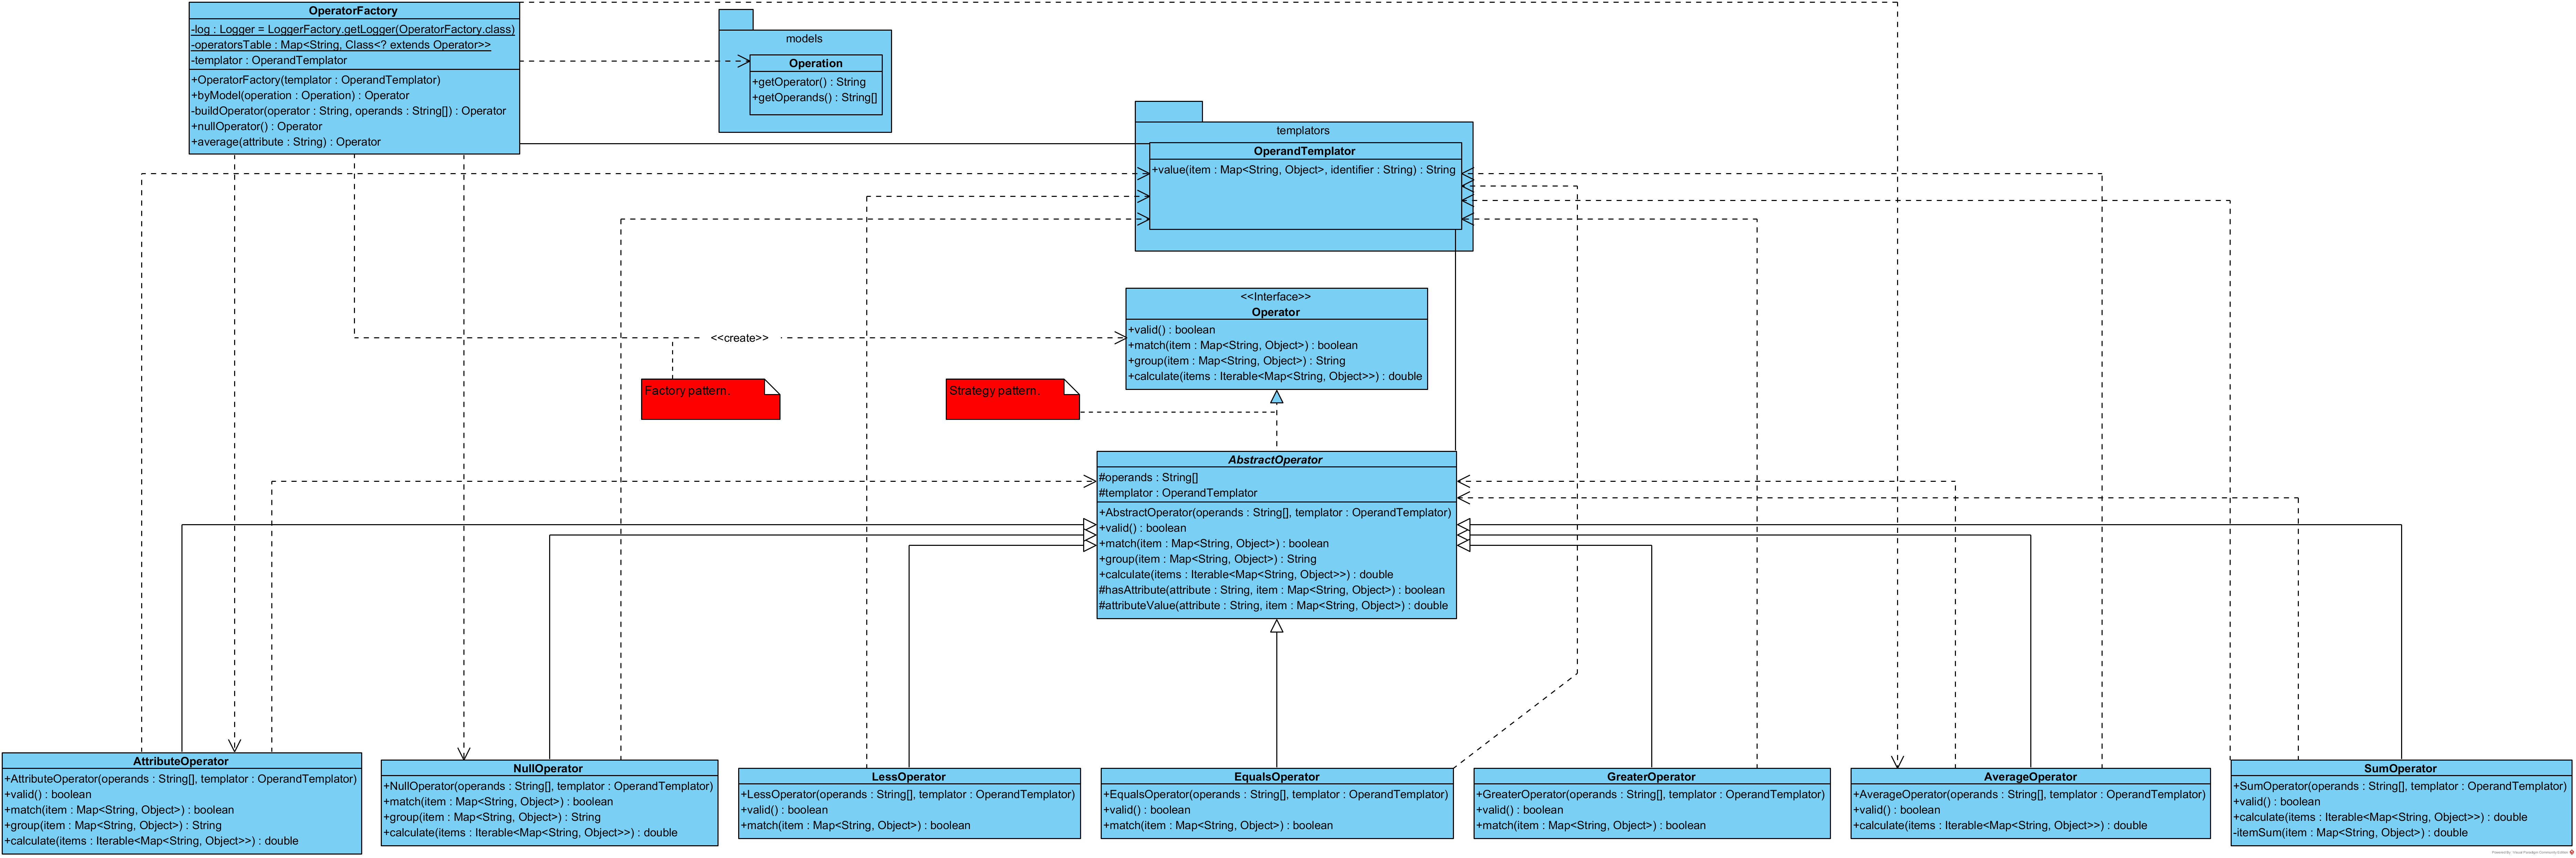
\includegraphics[width=\textwidth]{./img/DiagrammiClasse/operators.png}
            \caption[Diagramma del package operators]{Diagramma del package operators}
        \end{figure}
        Il diagramma rappresenta il package operators. In tale package sono contenute tutte le classi che rappresentano gli operatori che
        vengono utilizzati nelle operazioni di \ProjectName{}. \\
        Spiegazione:
        \begin{itemize}
        	\item \textbf{Operator}: questa interfaccia rappresenta operatori in grado di eseguire operazioni su oggetti,
        		\GroupName{} ha scelto di basarsi sullo strategy pattern, descritto precedentemente, per lo sviluppo di
        		questa classe e delle sue sotto classi, per rendere maggiormente estendibile il prodotto;
        	\item \textbf{AbstractOperator}: classe astratta con un'implementazione base di un operatore;
        	\item \textbf{AttributeOperator}: operatore per ottenere l'attributo di un oggetto;
        	\item \textbf{NullOperator}: operatore nullo che non effettua nessuna operazione o calcolo;
        	\item \textbf{LessOperator}: operatore per verificare che il primo operatore sia minore del secondo;
        	\item \textbf{EqualsOperator}: operatore per verificare che due valori siano uguali;
        	\item \textbf{GreaterOperator}: operatore per verificare che il primo operatore sia maggiore del secondo;
        	\item \textbf{AverageOperator}: operatore per calcolare la media di un attributo in un insieme di traces;
        	\item \textbf{SumOperator}: operatore che effettua la somma di un attributo in un insieme di oggetti.
        	\item \textbf{OperatorFactory}: classe che permette di costruire un operatore in base ad una 
        		configurazione scelta, \GroupName{} ha scelto di organizzare l'architettura di questa classe
        		seguendo il factory pattern, già descritto precedentemente;
        	\item \textbf{OperandTemplator}: classe utilizzata per gestire gli operandi nelle operazioni.
        \end{itemize}

\newpage

    \subsection{Package strategies}

        \begin{figure}[htbp]
            \centering
            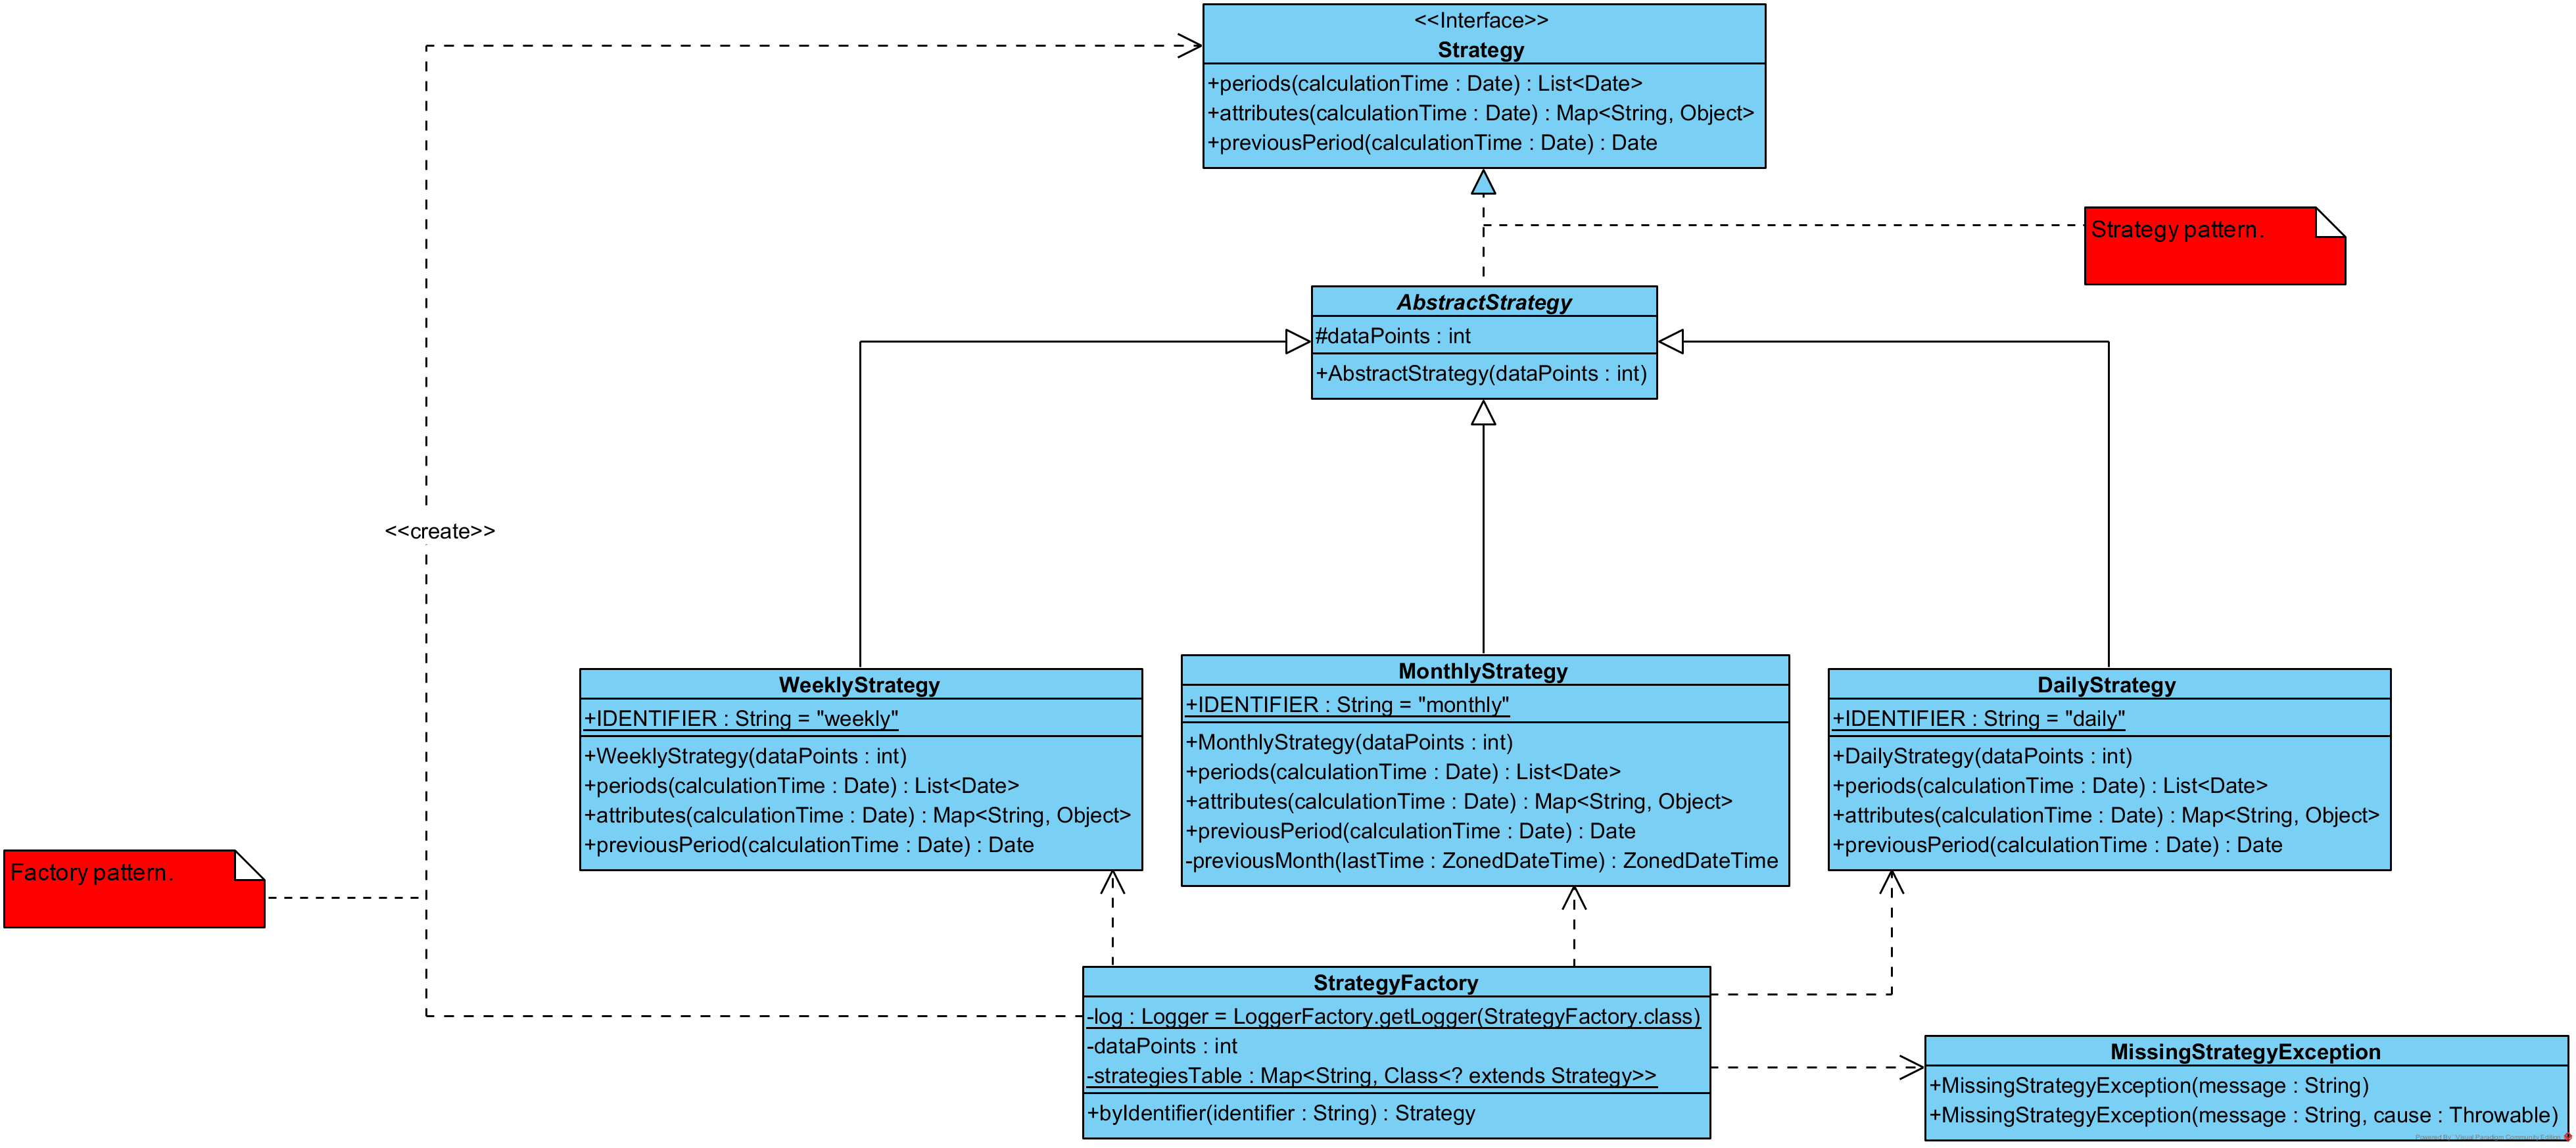
\includegraphics[width=\textwidth]{./img/DiagrammiClasse/Strategies.png}
            \caption[Diagramma del package strategies]{Diagramma del package strategies}
        \end{figure}
        Il diagramma rappresenta il package strategies composto dalle seguenti classi:
        \begin{itemize}
        	\item \textbf{Strategy}: interfaccia di una strategia per il calcolo di una baseline,
        		per rendere indipendente la strategia scelta del client che la utilizza è stato scelto
        		di organizzare queste classi basandosi sullo strategy pattern già visto precedentemente
        		anche in altre classi;
        	\item \textbf{AbstractStrategy}: classe astratta di una strategia che gestisce le proprietà di default;
        	\item \textbf{WeeklyStrategy}: classe per calcolare baseline su base settimanale.
        	\item \textbf{MonthlyStrategy}: classe per calcolare baseline su base mensile;
        	\item \textbf{DailyStrategy}: classe per calcolare baseline su base giornaliera;
        	\item \textbf{StrategyFactory}: classe che permette di costruire una strategia in base ad 
        		una configurazione scelta, questa classe si basa sul factory pattern per rendere indipendente 
        		l'oggetto utilizzato della sua effettiva implementazione; 
        	\item \textbf{MissingStrategyException}: eccezione lanciata quando non è possibile definire una 
        		strategia a causa di parametri in input non validi.
        \end{itemize}


